%Set the document class and font size
\documentclass[fleqn, bachelor,subf,12pt,notitlepage]{disser}

\usepackage[utf8]{inputenc}
\usepackage{enumerate}
\usepackage{amsmath}
\usepackage{mathtools} 
\usepackage{amssymb}
\usepackage{systeme}
\usepackage[english]{babel}
\usepackage{xparse}
\usepackage{xfrac}
\usepackage{setspace}
\usepackage{multicol}
\usepackage{array}
\usepackage{tabularx}
\usepackage{bigints}
\usepackage{fontspec}
\usepackage{fancyhdr}


%This is a command for creating new command for reducing the size of the given math equation
\newcommand\scalemath[2]{\scalebox{#1}{\mbox{\ensuremath{\displaystyle #2}}}}


\usepackage{geometry}
 \geometry
{
 	a4paper,
 	total={170mm,257mm},
 	left=30mm,
	right = 10mm,
 	top=20mm,
	bottom=25mm
 }

%\pagestyle{fancy}
%\fancyhead{}

\setmainfont{GHEA Grapalat}
\onehalfspacing

\title{Դիպլոմային աշխատանք}
\author{Կամո Սևոյան}
\date{}

\begin{document}

\section*{Ներածություն}
\subsection*{Հերմիթյան ինտերպոլյացիա}


Նախքան անդրադառնալը բազմաչամ ինտերպոլյացիայի խնդրին, քննարկենք մեկ փոփոխականի ֆունկցիայի ինտերպոլյացիայի որոշ դետալներ։ 

Ենթադրենք տրված են $f:\Omega \mapsto \Theta, \Omega, \Theta \subset \mathbb{R}$ ֆունկցիան,  $\left\{x_{i}\right\}_{i=0}^{N}$ կետերը և դրանց համապատասխան $\left\{y_{i}=f\left(x_{i}\right)\right\}_{i=0}^{N}$ արժեքները։ Յուրաքանչյուր $\left[x_{i}, x_{i+1}\right]$ հատվածում \newline ինտերպոլացնող ֆունկցիան իրենից ներկայացնում է գխային ֆունկցիա, որը կարելի է ներկայացնել հետևյալ տեսքով.

$$p_{1}^{(i)}\left(x\right)=\dfrac{x_{i+1}-x}{x_{i+1}-x_{i}}y_{i}+\dfrac{x-x_{i+1}}{x_{i+1}-x_{i}}y_{i+1}, i=\overline{0, N-1}$$

Այսպիսով $\left[x_{0}, x_{N}\right]$ հատվածում կտոր առ կտոր մոտարկող ֆունկցիան տրվում է հետևյալ կերպ.

$$p_{1}\left(x\right)=\sum_{i=0}^{N}\varphi_{i} \left(x\right)y_{i}$$

Որտեղ 

\begin{align*}
\varphi_{0}\left(x\right)&=\begin{cases}
\dfrac{x_{1}-x}{x_{1}-x_{0}}, x\in \left[x_{0}, x_{1}\right]\\
0, x\in \left[x_{1}, x_{N}\right]\\
\end{cases}\\
\varphi_{i}\left(x\right)&=\begin{cases}
0, x\in \left[x_{0}, x_{i-1}\right]\\
\dfrac{x-x_{i-1}}{x_{i}-x_{i-1}}, x\in \left[x_{i-1}, x_{i}\right]\\
\dfrac{x_{i+1}-x}{x_{i+1}-x_{i}}, x\in \left[x_{i}, x_{i+1}\right]\\
0, x\in \left[x_{i+1}, x_{N}\right]\\
\end{cases}\\
\varphi_{N}\left(x\right)&=\begin{cases}
0, x\in \left[x_{0}, x_{N-1}\right]\\
\dfrac{x-x_{N-1}}{x_{N}-x_{N-1}}, x\in \left[x_{N-1}, x_{N}\right]\\
\end{cases}
\end{align*}

$\varphi_{i}\left(x\right)$ ֆունկցիաները կոչվում են բազիսային ֆունկցիաներ, որոնք ունեն այսպես կոչված լոկալ կրողներ, քանի որ դրանք ոչ զրոյական են որևէ տիրույթում և զրոյական որոշման տիրույթի մնացած մասերում։
Նմանատիպ բազիսային ֆունկցիաների հիմնական հատկությունն այն է, որ դրանք հավասար են մեկի որևէ կոնկրետ հանգույցում և հավասար են զրոյի մնացած բոլոր հանգույցներում։ Նշենք սակայն, որ այս տիպի ինտերպոլյացիան $C^{0}$ դասի է, այսինք միայն անընդհատ է, և հետևաբար կիրառելի չէ այն խնդիրներում, որտեղ պահանջվում է ավելի բարձր կարգի ողորկություն։


\newpage

Ստորև տրված է բազիսային ֆունկցիաների սխեմատիկ ներկայացում.
\begin{figure}[h!]
\centering
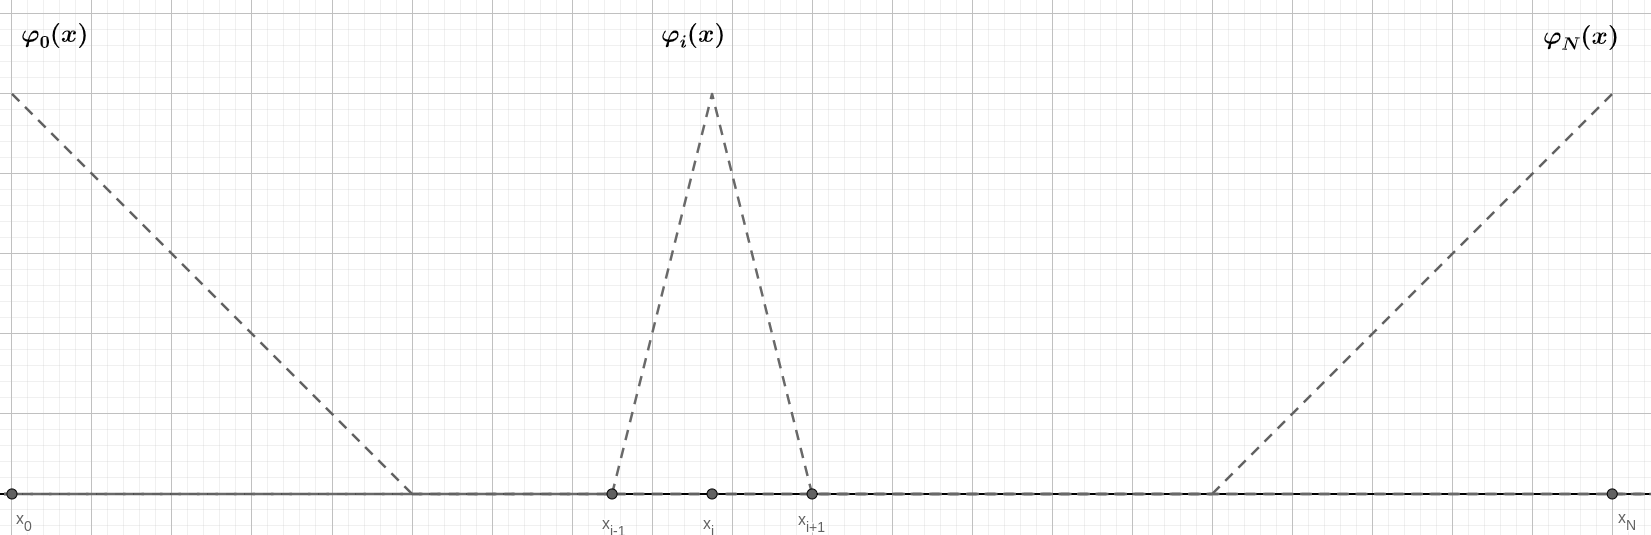
\includegraphics[width=1.0\textwidth]{images/one_var_linear}
\captionsetup{labelformat=empty}
\caption{\hfill Նկար 1}
\end{figure}


\newpage

Այժմ դիտարկենք հետևյալ խնդիրը.
Անհրաժեշտ է կառուցել  կտոր առ կտեր մոտարկող ֆունկցիա, որը ֆունկցիայի արժեքի հետ մեկտեղ կհամըկնի նաև ֆունկցիայի առաջին կարգի ածանցյալի հետ ինտերպոլյացիոն կետերում։ Այսինքն.

$$ \dfrac{d^{j}}{dx^j}f(x_{i})=\dfrac{d^{j}}{dx^j}p_{3}(x_{i}),   \; j=0, 1;  \; i=\overline{0, N-1}$$

Յուրաքանչյուր $\left[x_{i}, x_{i+1}\right]$ հատվածում ինտերպոլյացիոն ֆունկցիան իրենից ներկայացնում է խորանարդային ֆունկցիա, որը կարելի է ներկայացնել հետևյալ տեսքով։

$$p_{3}^{\left(i\right)} = \alpha_{i}(x)f(x_{i})+\beta_{i+1}(x)f(x_{i+1})+\gamma_{i}(x)f^{'}(x_{i})+\delta_{i+1}(x)f^{'}(x_{i+1})$$

որտեղ 

$$\alpha_{i}(x)=\dfrac{\left(x_{i+1}-x\right)^{2}\left[\left(x_{i+1}-x_{i}\right)+2\left(x-x_{i}\right)\right]}{\left(x_{i+1}-x_{i}\right)^{3}}, \beta_{i+1}(x)=\dfrac{\left(x-x_{i}\right)^{2}\left[\left(x_{i+1}-x_{i}\right)+2\left(x_{i+1}-x\right)\right]}{\left(x_{i+1}-x_{i}\right)^{3}}$$

$$\gamma_{i}(x)=\dfrac{\left(x-x_{i}\right)\left(x_{i+1}-x\right)^{2}}{\left(x_{i+1}-x_{i}\right)^{2}}, \delta_{i+1}(x)=\dfrac{\left(x-x_{i}\right)^2\left(x-x_{i+1}\right)}{\left(x_{i+1}-x_{i}\right)^{2}}$$

Այսպիսով $\left[x_{0}, x_{N}\right]$ հատվածում կտոր առ կտոր մոտարկող ֆունկցիան տրվում է հետևյալ կերպ.

$$p_{3}(x)=\sum_{i=0}^{N}\left[\varphi_{i}^{(0)}f(x_{i})+\varphi_{i}^{(1)}f^{'}(x_{i})\right]$$
որտեղ 
\begin{align*}
\varphi^{(0)}_{0}\left(x\right)&=\begin{cases}
\dfrac{\left(x_{1}-x\right)^{2}\left[\left(x_{1}-x_{0}\right)+2\left(x-x_{0}\right)\right]}{\left(x_{1}-x_{0}\right)^{3}},  x\in \left[x_{0}, x_{1}\right]\\
0, x\in \left[x_{1}, x_{N}\right]\\
\end{cases}\\
\varphi^{(0)}_{i}\left(x\right)&=\begin{cases}
0, x\in \left[x_{0}, x_{i-1}\right]\\
\dfrac{\left(x-x_{i-1}\right)^{2}\left[\left(x_{i}-x_{i-1}\right)+2\left(x_{i}-x\right)\right]}{\left(x_{i}-x_{i-1}\right)^{3}}, x\in \left[x_{i-1}, x_{i}\right]\\
\dfrac{\left(x_{i+1}-x\right)^{2}\left[\left(x_{i+1}-x_{i}\right)+2\left(x-x_{i}\right)\right]}{\left(x_{i+1}-x_{i}\right)^{3}}, x\in \left[x_{i}, x_{i+1}\right]\\
0, x\in \left[x_{i+1}, x_{N}\right]\\
\end{cases}\\
\varphi^{(0)}_{N}\left(x\right)&=\begin{cases}
0, x\in \left[x_{0}, x_{N-1}\right]\\
\dfrac{\left(x-x_{N-1}\right)^{2}\left[\left(x_{N}-x_{N-1}\right)+2\left(x_{N}-x\right)\right]}{\left(x_{N}-x_{N-1}\right)^{3}}, x\in \left[x_{N-1}, x_{N}\right]\\
\end{cases}
\end{align*}

\begin{align*}
\varphi^{(1)}_{0}\left(x\right)&=\begin{cases}
\dfrac{\left(x-x_{0}\right)\left(x_{1}-x\right)^{2}}{\left(x_{1}-x_{0}\right)^{2}}, x\in \left[x_{0}, x_{1}\right]\\
0, x\in \left[x_{1}, x_{N}\right]\\
\end{cases}\\
\varphi^{(1)}_{i}\left(x\right)&=\begin{cases}
0, x\in \left[x_{0}, x_{i-1}\right]\\
\dfrac{\left(x-x_{i-1}\right)^2\left(x-x_{i}\right)}{\left(x_{i}-x_{i-1}\right)^{2}}, x\in \left[x_{i-1}, x_{i}\right]\\
\dfrac{\left(x-x_{i}\right)\left(x_{i+1}-x\right)^{2}}{\left(x_{i+1}-x_{i}\right)^{2}}, x\in \left[x_{i}, x_{i+1}\right]\\
0, x\in \left[x_{i+1}, x_{N}\right]\\
\end{cases}\\
\varphi^{(1)}_{N}\left(x\right)&=\begin{cases}
0, x\in \left[x_{0}, x_{N-1}\right]\\
\dfrac{\left(x-x_{N-1}\right)^{2}\left(x-x_{N}\right)}{\left(x_{N}-x_{N-1}\right)^{2}}, x\in \left[x_{N-1}, x_{N}\right]\\
\end{cases}
\end{align*}

Ստորև տրված է բազիսային ֆունկցիաների սխեմատիկ ներկայացում.
\begin{figure}[h!]
\centering
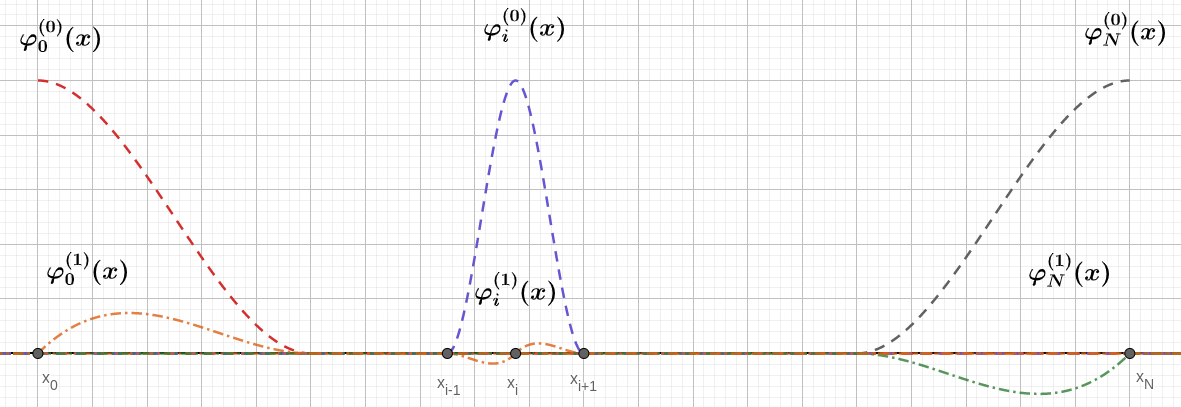
\includegraphics[width=1.0\textwidth]{images/one_var_quadratic}
\captionsetup{labelformat=empty}
\caption{\hfill Նկար 2}
\end{figure}

Այսպիսով ստացանք $C^{1}$ ինտերպոլյացիա։

Ընդհանուր դեպքում հերմիթյան ինտերպոլյացիայի պայմանը կարելի է գրել հետևյալ կերպ.
$$\dfrac{d^{k}}{dx^{k}}f\left(x_{i}\right)=\dfrac{d^{k}}{dx^{k}}p_{2m-1}\left(x_{i}\right), \;  i=\overline{0, N}, \;  k=\overline{0, m-1}$$

\newpage

\subsection*{Քառակուսային և խորանարդային ինտերպոլյացիա}

Խնդիրներում, որտեղ անհրաժեշտ է որոշել միայն տրված ֆունկիցիան, ֆունկցիայի ածանցյալներն ինտերպոլացնելու փոխարեն դրվում է դրանց անընդհատության պայման բազիսային ֆուկցիաների միացման կետերում,  բավականին հեշտացնելով դրված խնդիրը և դրա լուծումը։ Սակայն այս դեպքում բազիսային ֆունկցիաները չեն հանդիսանում լոկալ կրողներ, ուստի կիրառական տեսանկյունից հարմար չեն։

Նման տիպի ինտերպոլյացիայի կառուցման պարզագույն օրինակը հետևյալն է.

\noindent Յուրաքանչյուր $\left[x_{i}, x_{i+1}\right]$ ինտերվալում կառուցենք այպիսի պարաբոլ, որ բոլոր $x_{i}$ հանգուցային կետերում առանջին կարգի ածանցյալները լինեն անընդհատ։

$$S_{2}^{(i)}(x)=f(x_{i})+\dfrac{f(x_{i+1})-f(x_{i})}{x_{i+1}-x_{i}}\left(x-x_{i}\right)+c_{i}\left(x-x_{i}\right)\left(x-x_{i+1}\right)$$

\noindent Ածանցյալների անընդհատության պայմանից կհետևի, որ

$$c_{i}+c_{i-1}=\dfrac{1}{h^{2}}\left(f(x_{i+1})-2f(x_{i})+f(x_{i-1})\right) \; i=\overline{1, N-1}$$

Քանի որ համակարը պարունակում է $N-1$ հավասարում, ապա մնում է մեկ ազատ գործակից, որը կարելի գտնել, որևէ $x_{j}$ հանգուցային կետում որոշելով $S_{2}^{(j)''}$֊ն։
%TODO: Add some equations and a plot


Առավել կիրառելի են խորանարդային սփլայնները։ Այս դեպքում յուրաքանչյուր $\left[x_{i}, x_{i+1}\right]$ ինտերվալում կառուցվում են երրորդ աստիճանի բազմանդամներ այնպիսին, որ դրանց միացման կետերում (հանգույցներում) առաջին և երկրորդ կարգի ածանցյալները լինեն անընդհատ։ 

Բազմանդամը դիտարկելու փոխարեն դիտարկենք նրա երկրորդ կարգի ածանցյալը: Այն գծային ֆունկցիա է, հետևաբար այն կարելի է ներկայացնել հետևյալ տեսքով.

$$ S^{(i)''}_3(x)=c_{i}\dfrac{x_{i+1}-x}{x-x_{i}}+c_{i+1}\dfrac{x-x_{i}}{x_{i+1}-x_{i}}$$

\noindent որտեղ $c_{i}$ և $c_{i+1}$֊ը $x_{i}$ և $x_{i+1}$ կետերում երկրորդ կարգի ածանցյալների արժենքներն են։ 
\noindent Հաշվի առնելով նաև հետևյալ պայմանները.

$$\begin{cases}
				S_{3}^{(i)}(x_{i}) &=f_{i}\\
				S_{3}^{(i)}(x_{i+1}) &= f_{i+1}\\
				S_{3}^{(i-1)'}(x_{i}) &= S_{3}^{(i)'}(x_{i})

\end{cases}
$$

\noindent կստանանք հետևյալ տեսքի խորանարդային սփլայն.

$$
	S_{3}^{(i)}(x) = \dfrac{c_{i}}{6h}\left(x_{i+1}-x\right)^{3}+\dfrac{c_{i+1}}{6h}\left(x-x_{i}\right)^{3}+\left(\dfrac{f_{i}}{h}-\dfrac{hc_{i}}{6}\right)\left(x_{i+1}-x\right)+\left(\dfrac{f_{i+1}}{h}-\dfrac{hc_{i+1}}{6}\right)\left(x-x_{i}\right)
$$

$c_{i}$ գործակիցները բավարարում են հետևյալ պայմաններին.

$$c_{i+1}+4c_{i}+c_{i-1} = \dfrac{6}{h^2}\left(f_{i+1}-2f_{i}+f_{i-1}\right)$$

Ստորև ներկայացվում է քառակուսային և խորանարդային ինտերպոլյացիայի օրինակ
\begin{figure}[h!]
\centering
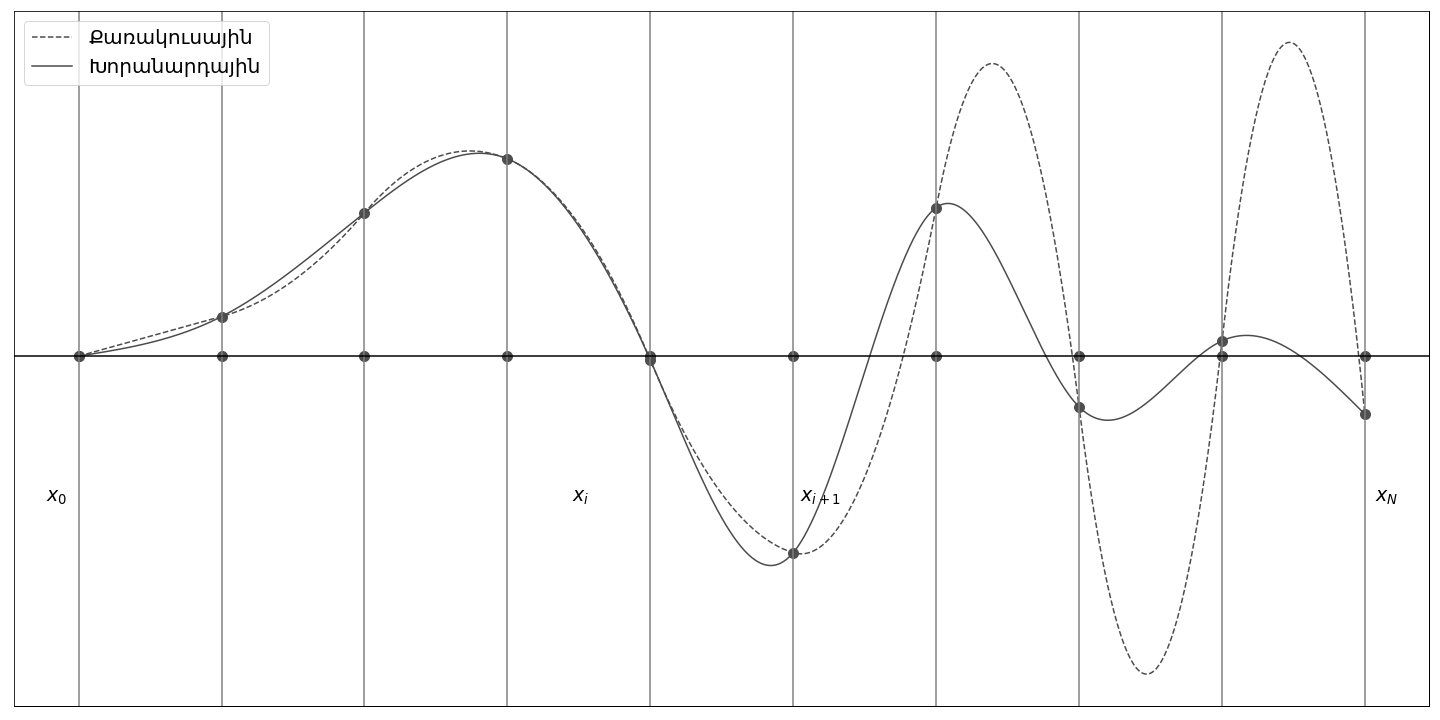
\includegraphics[width=1.0\textwidth]{images/quadratic_and_cubic_interploation}
\captionsetup{labelformat=empty}
\caption{\hfill Նկար N}
\end{figure}

\newpage
Այժմ դիտարկենք լոկալ կրող ունեցող խորանարդային սփլայները։ Այդպիսի սփլայ առաջարկել է ավստրացի մաթեմատիկոս Առնոլդ Շնեբերգը։

Դիտարկենք հետևյալ ֆունկցիան.

$$\gamma(x)=\dfrac{1}{4}\left[\left(x+2\right)^{3}_{+} - 4\left(x+1\right)^{3}_{+}+ \left(x\right)^{3}_{+} -4\left(x-1\right)^{3}_{+} + \left(x-2\right)^{3}_{+}\right]$$
 Ստորև ներկայացվում է $\gamma$ ֆունկցիան և նրա մինչև երրորդ կարգի ածանցյալները.
\begin{figure}[h!]
\centering
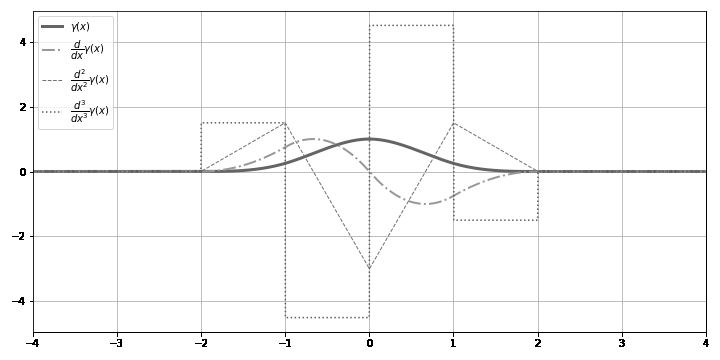
\includegraphics[width=1.0\textwidth]{images/cubic_compact_support_basis}
\captionsetup{labelformat=empty}
\caption{\hfill Նկար 3}
\end{figure}

Ենթադրենք տրված է $\left[x_{0}, x_{N}\right]$ ինտերվալը, և տրոհված է $N$ հավասար մասերի h քայլով։ Յուրաքանչյուր հանգուցային կետի $(i=2, \dots N-2)$ համար բազիսային ֆունկցիան տրվում է հետևյալ բանաձևով.

					$$B_{i}\left(\dfrac{x}{h}\right)=\gamma \left(\frac{x-x_{0}}{h}-i\right)$$
Այս ֆունկցիաները և նրանց մինչև երկրորդ կարգի ածանցյալները հավասար են զրոյի $\mathbb{R} \textbackslash \left[x_{i-2}, x_{i+2}\right]$ տիրույթում։

Մնացած բազիսային ֆունկիաները պետք է կառուցել այլ կերպ, քանի որ դրանց մի մասը դուրս է ըկած  $\left[x_{0}, x_{N}\right]$ ինտերվալից։

$$B_{0}\left(\frac{x}{h}\right) = \gamma \left(\frac{x}{h}\right) + \left(\dfrac{h - x}{4h}\right)^{3}_{+} , \; x \in \left[x_{0}, x_{2}\right]$$
$$B_{1}\left(\frac{x}{h}\right) = \gamma \left(\frac{x}{h}\right), \; x \in \left[x_{0}, x_{3}\right]$$
$$B_{N-1}\left(\frac{x}{h}\right) = \gamma \left(\frac{x}{h}\right), \; x \in \left[x_{N-3}, x_{N}\right]$$
$$B_{N}\left(\frac{x}{h}\right) = \gamma \left(\frac{x}{h}\right) + \left(\dfrac{x - (N-1)h}{4h}\right)^{3}_{+} , \; x \in \left[x_{N-2}, x_{N}\right]$$

Ստորև ներկայացվում է $B_{j}$ բազիսների գծագիրը.

\begin{figure}[h!]
\centering
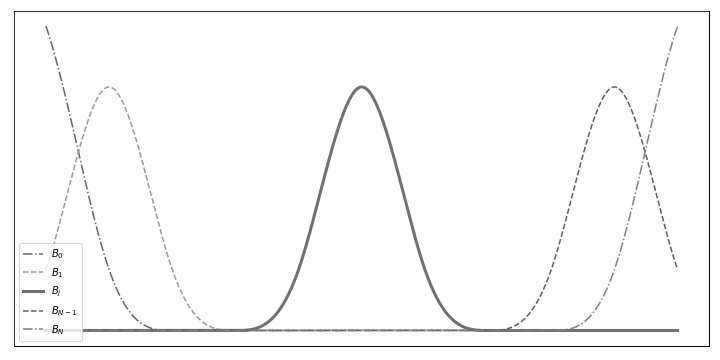
\includegraphics[width=1.0\textwidth]{images/all_cubic_compact_support_basis}
\captionsetup{labelformat=empty}
\caption{\hfill Նկար 3}
\end{figure}

Տրված $\left\{f_{j}\right\}$ ինտերպոլյացիոն տվյալնեով կառուցենք սփլայն.

				$$ F(x) = \sum_{i=0}^{N} \alpha_{i}B_{i}\left(\frac{x}{h}\right)$$

Հաշվի առնելով ինտերպոլյացիոն պայմանները.

				$$F(x_{i}) = f_{i}$$

կստանանք հետևյալ հավասարումերի համակարգը.
 
$$\begin{dcases}
\frac{5}{4}\alpha_{0} + \frac{1}{4}\alpha_{0} &= f_{0}\\
\frac{1}{4}\alpha_{j-1} + \alpha_{j} + \frac{1}{4}\alpha_{j+1} &= f_{j}\\
\frac{5}{4}\alpha_{N-1} + \frac{1}{4}\alpha_{N} &= f_{N}\\
\end{dcases}$$
\newpage
\section*{Երկչափ մոտարկում}

Այժմ դիտարկենք երկու փոփոխականի կտոր առ կտոր անընդհատ մոտարկման խնդիրը $\partial R$ եզրով սահմանափակ $R$ տիրությում։ Տիրույթը տրոհվում է որոշակի թվով էլեմենտների։ Կախված $R$ տիրույթից, առանձնացվում են հետևյալ մոտակման ձևերը.

\subsection*{Ուղղանկյուն տիրույթ}

Դիցուք տրված են $f:\Omega\mapsto \Theta$,  $\Theta \subset \mathbb{R}$, $\Omega \subset \mathbb{R}^{2} = \left[x_{0}, x_{M}\right] \times \left[y_{0}, y_{N}\right]$,  ուղղանկյուն տիրույթը, որը տրոհված է $\left[x_{i}, x_{i+1}\right] \times \left[y_{j}, y_{j+1}\right]$, ուղղանկյուն էլեմենտների:
$$x_{i+1}-x_{i}=h_{1}, \; y_{j+1}-y_{j}=h_{2}, \; i=\overline{0, M-1}, j=\overline{0, N-1}$$

\begin{figure}[h!]
\centering
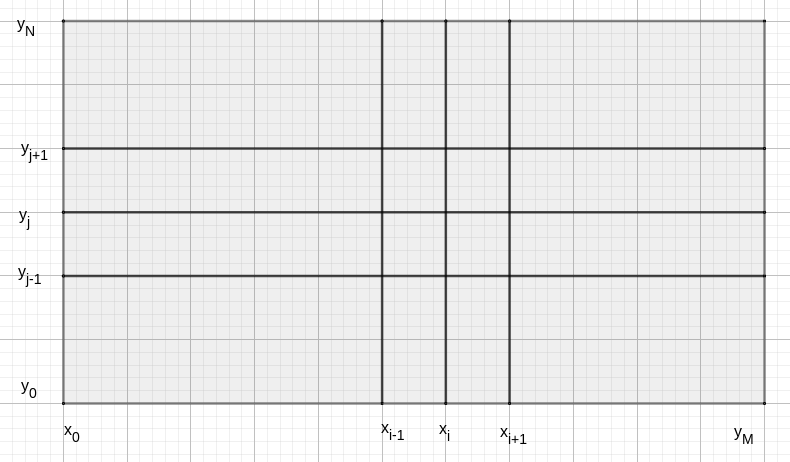
\includegraphics[width=0.6\textwidth]{images/two_var_linear}
\captionsetup{labelformat=empty}
\caption{\hfill Նկար 3}
\end{figure}

\subsubsection*{$C^{(0,0)}$ մոտարկում}


Յուրաքանչյուր  $\left[x_{i}, x_{i+1}\right] \times \left[y_{j}, y_{j+1}\right]$ էլեմենտի վրա $f$ ֆունկցիան մոտարկվում հետևյալ քառակուսային ֆունկցիայով։

$$\scalemath{0.9}{p_{1}^{(i, j)}(x, y)=\alpha_{i,j}(x,y)f(x_{i},y_{j})+\beta_{i+1,j}(x,y)f(x_{i+1},y_{j})\scalemath{0.2}+\gamma_{i,j+1}(x,y) f(x_{i},y_{j+1})+\delta_{i+1, j+1}(x,y)f(x_{i+1},y_{j+1})}$$
 որտեղ 

$$\alpha_{i,j}(x,y)=\dfrac{1}{h_{1}h_{2}}\left(x_{i+1}-x\right)\left(y_{j+1}-y\right)$$
$$\beta_{i+1,j}(x,y)=\dfrac{1}{h_{1}h_{2}}\left(x-x_{i}\right)\left(y_{j+1}-y\right)$$
$$\gamma_{i,j+1}(x,y)=\dfrac{1}{h_{1}h_{2}}\left(x_{i+1}-x\right)\left(y-y_{j}\right)$$
$$\delta_{i+,j+1}(x,y)=\dfrac{1}{h_{1}h_{2}}\left(x-x_{i}\right)\left(y-y_{j}\right)$$

Այսպիսով $\left[x_{0}, x_{M}\right] \times \left[y_{0}, y_{M}\right]$ տիրույթում կտոր առ կտոր մոտարկող ֆունկցիան տրվում է հետևյալ կերպ.

$$p_{1}(x,y)=\sum_{i=0}^{m}\sum_{j=0}^{n}\varphi_{i,j}(x,y)f(x_{i},y_{j})$$
որտեղ

%TODO: change 'otherwise' to armenian one, at this moment this is not possible because XeLaTeX can not render armenian letter in math equations

$$\varphi_{i,j}\left(x, y\right)=\begin{dcases}
\dfrac{1}{h_{1}h_{2}}\left(x-x_{i-1}\right)\left(y-y_{j-1}\right), (x,y)\in \left[x_{i-1}, x_{i}\right]\times\left[y_{j-1}, y_{j}\right]\\
\dfrac{1}{h_{1}h_{2}}\left(x-x_{i-1}\right)\left(y_{j+1}-y\right), (x,y)\in \left[x_{i-1}, x_{i}\right]\times\left[y_{j}, y_{j+1}\right]\\
\dfrac{1}{h_{1}h_{2}}\left(x_{i+1}-x\right)\left(y-y_{j-1}\right), (x,y)\in \left[x_{i}, x_{i+1}\right]\times\left[y_{j-1}, y_{j}\right]\\
\dfrac{1}{h_{1}h_{2}}\left(x_{i+1}-x\right)\left(y_{j+1}-y\right), (x,y)\in \left[x_{i}, x_{i+1}\right]\times\left[y_{j}, y_{j+1}\right]\\
0, otherwise\\
\end{dcases}$$

Վերը դիտարկված մոտարկումը հանդիսանում է երկչափ Հերմիթյան մոտարկման մասնավոր դեպք։

Ընդհանուր դեպքում, տրված $k\in \mathbb{N}$ թվի և տրված ուղղանկյուն տիրույթի ցանկացած ուղղանկյունաձև տրոհման էլեմենտում կարելի է կառուցել $C^{k-1, k-1}$ կարգի մոտարկող բազմանդամ, որը $2k-1$ ֊րդ կարգի բազմանդամ է ըստ իր յուրաքանչյուր փոփոխականի և, ինտերպոլյացիայի պայմանները կարելի է գրել հետևյալ կերպ.

$$ \dfrac{d^{p+q}}{dx^p dy^{q}}f(x_{i}, y_{j})=\dfrac{d^{p+q}}{dx^{p}dy^{q}}p_{2k-1}(x_{i}, y_{j})$$
$$p, q = \overline{0, k-1}; \; i=\overline{0, M};  \;  j=\overline{0, N}$$


\newpage

\noindent Այժմ դիտարկենք ուղղանկյուն տիրույթի տրոհման և բազիսային ֆունկցիաների կառուցման այլ տարբերակ։ Այս դեպքում տիրույթը տրոհենք ըստ նախորդ տարբերակի, ի հավելումն յուրաքանչյուր ուղղանկյուն էլեմենտ տրոհելով երկու ուղղանկյուն եռանկյունների.

Դիտարկենք հետևյալ ֆունկցիան.

$$\varphi \left(x,y\right)=\begin{cases}
1-y, &(x,y) \in S_{1} \\
1+x-y, &(x,y) \in S_{2} \\
1+x, &(x,y) \in S_{3} \\
1+y, &(x,y) \in S_{4} \\
1-x+y, &(x,y) \in S_{5} \\
1-x, &(x,y) \in S_{6}\\
0, otherwise
\end{cases} $$


\begin{figure}[h!]
  \centering
  \begin{minipage}[b]{0.4\textwidth}
    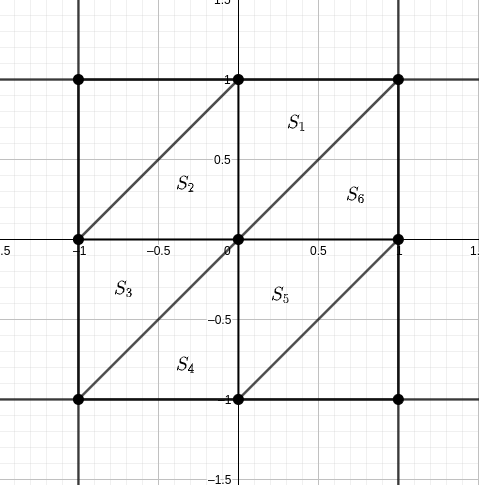
\includegraphics[width=\textwidth]{images/two_var_courant_1}
    \captionsetup{labelformat=empty}
    \caption{Նկար 4}
  \end{minipage}
  \hfill
  \begin{minipage}[b]{0.4\textwidth}
    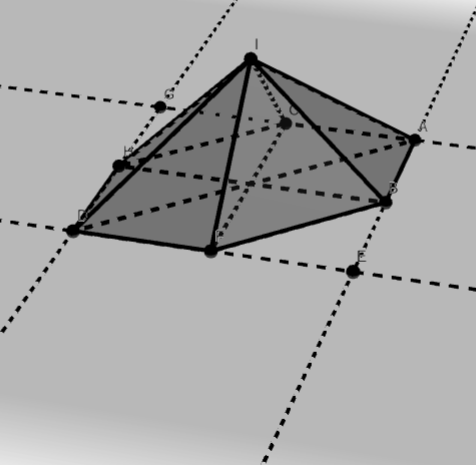
\includegraphics[width=\textwidth]{images/two_var_courant_2}
    \captionsetup{labelformat=empty}
    \caption{Նկար 5}
  \end{minipage}
\end{figure}

\noindent Պարզ է, որ այն յուրաքանչյուր ուղղանկյուն էլեմենտում $C^{(0, 0)}$ ֆունկցիա է:

\noindent  Այժմ յուրաքանչյուր $x_{i}, y_{j}$ կետի վրա կառուցենք հետևյալ ֆունկցիան.

$$\varphi_{i,j}(x,y)=\varphi \left(\dfrac{x-x_{i}}{h_{1}}, \dfrac{y-y_{j}}{h_{2}}\right)$$

\newpage

Այդ դեպքում $f$ ֆունկցիայի մոտարկման բանաձևը կտվրի հետևյալ կերպ։

$$p_{1}(x,y)=\sum_{i=0}^{N}\sum_{j=0}^{M}\varphi_{i,j}(x,y)f(x_{i}, y_{j})$$

\begin{figure}[h!]
\centering
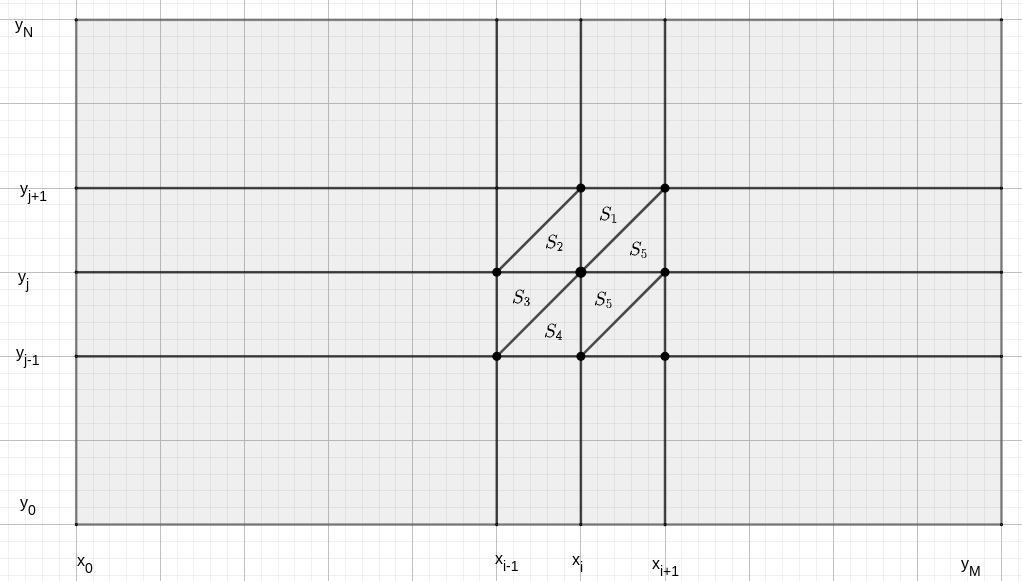
\includegraphics[width=0.6\textwidth]{images/two_var_courant_3}
\captionsetup{labelformat=empty}
\caption{\hfill Նկար 5}
\end{figure}

\newpage
\subsubsection*{$C^{(2,2)}$ մոտարկում}
Մեկ փոփոխականի մոտարկան խնդրը դիտարկելից քննարկեցինք Շներբերգի կողմից առաջարկված խորանարդային բազիսային սփլայնները։ Այս սփլայնները կարող ենք \newline օգտագործել երկչափ մոտարկման համար։
Յուրաքանչյուր $\left(x_{i}, y_{j}\right)$ հանգույցի վրա կառուցենք բազիսային ֆունկցիա կազմելով $B_{i}\left(\dfrac{x}{h_{1}}\right)$ և $B_{j}\left(\dfrac{x}{h_{2}}\right)$ ֆունկցիաների թենզորական \newline արտադրյալը։

		$$\varphi^{ij}\left(x, y\right) = B_{i}\left(\dfrac{x}{h_{1}}\right) B_{j}\left(\dfrac{x}{h_{2}}\right)$$

\noindent Տրված $\left\{f_{ij}\right\}$ ինտերպոլյացիոն տվյալնեով կառուցենք սփլայն.

				$$ F(x,y) = \sum_{i=0}^{N} \alpha_{ij}\varphi^{ji}\left(x, y\right)$$

\noindent Հաշվի առնելով ինտերպոլյացիոն պայմանները.

				$$F(x_{ij}) = f_{ij}$$

\noindent կստանանք հետևյալ հավասարումերի համակարգը.
 
$$\begin{dcases}
\alpha_{00}+\frac{5}{16}(\alpha_{01} + \alpha_{10}) +\frac{1}{16}\alpha_{11} &= f_{00}\\
\alpha_{M0}+\frac{5}{16}(\alpha_{M1} + \alpha_{M-1,0}) +\frac{1}{16}\alpha_{M-1, 1} &= f_{M0}\\
\alpha_{0N}+\frac{5}{16}(\alpha_{1N} + \alpha_{0,N-1}) +\frac{1}{16}\alpha_{N-1, 1} &= f_{0N}\\
\alpha_{MN}+\frac{5}{16}(\alpha_{M-1,N} + \alpha_{M,N-1}) +\frac{1}{16}\alpha_{M-1,N-1} &= f_{MN}\\
\frac{5}{4}\alpha_{i,1}+\frac{5}{16}(\alpha_{i-1,0} + \alpha_{i+1,0}) +\frac{1}{4}\alpha_{i,1} + \frac{1}{16}(\alpha_{i-1,1}+\alpha_{i+1,1}) &= f_{i0}\\
\frac{5}{4}\alpha_{i,N-1}+\frac{5}{16}(\alpha_{i-1,N} + \alpha_{i+1,N}) +\frac{1}{4}\alpha_{i,N-1} + \frac{1}{16}(\alpha_{i-1,N-1}+\alpha_{i+1,N-1}) &= f_{iN}\\
\frac{5}{4}\alpha_{1,j}+\frac{5}{16}(\alpha_{0,j-1} + \alpha_{0,j+1}) +\frac{1}{4}\alpha_{1,j} + \frac{1}{16}(\alpha_{1,j-1}+\alpha_{1,j+1}) &= f_{0j}\\
\frac{5}{4}\alpha_{M-1,j}+\frac{5}{16}(\alpha_{M,j-1} + \alpha_{M,j+1}) +\frac{1}{4}\alpha_{M-1,j} + \frac{1}{16}(\alpha_{M-1,j-1}+\alpha_{M-1,j+1})& = f_{Mj}\\
\alpha_{ij} + \frac{1}{4}(\alpha_{i,j-1} + \alpha_{i,j+1} + \alpha_{i-1,j} + \alpha_{i+1,j}) + \frac{1}{16}(\alpha_{i-1,j-1} + \alpha_{i-1,j+1} + \alpha_{i+1,j-1} +\alpha_{i+1,j+1}) &= f_{ij}
\end{dcases}$$

\newpage
Ստորև ներկայացվում է $\varphi^{ij}$ բազիսային ֆունկցիաների գծագիրը.

\begin{figure}[h!]
\centering
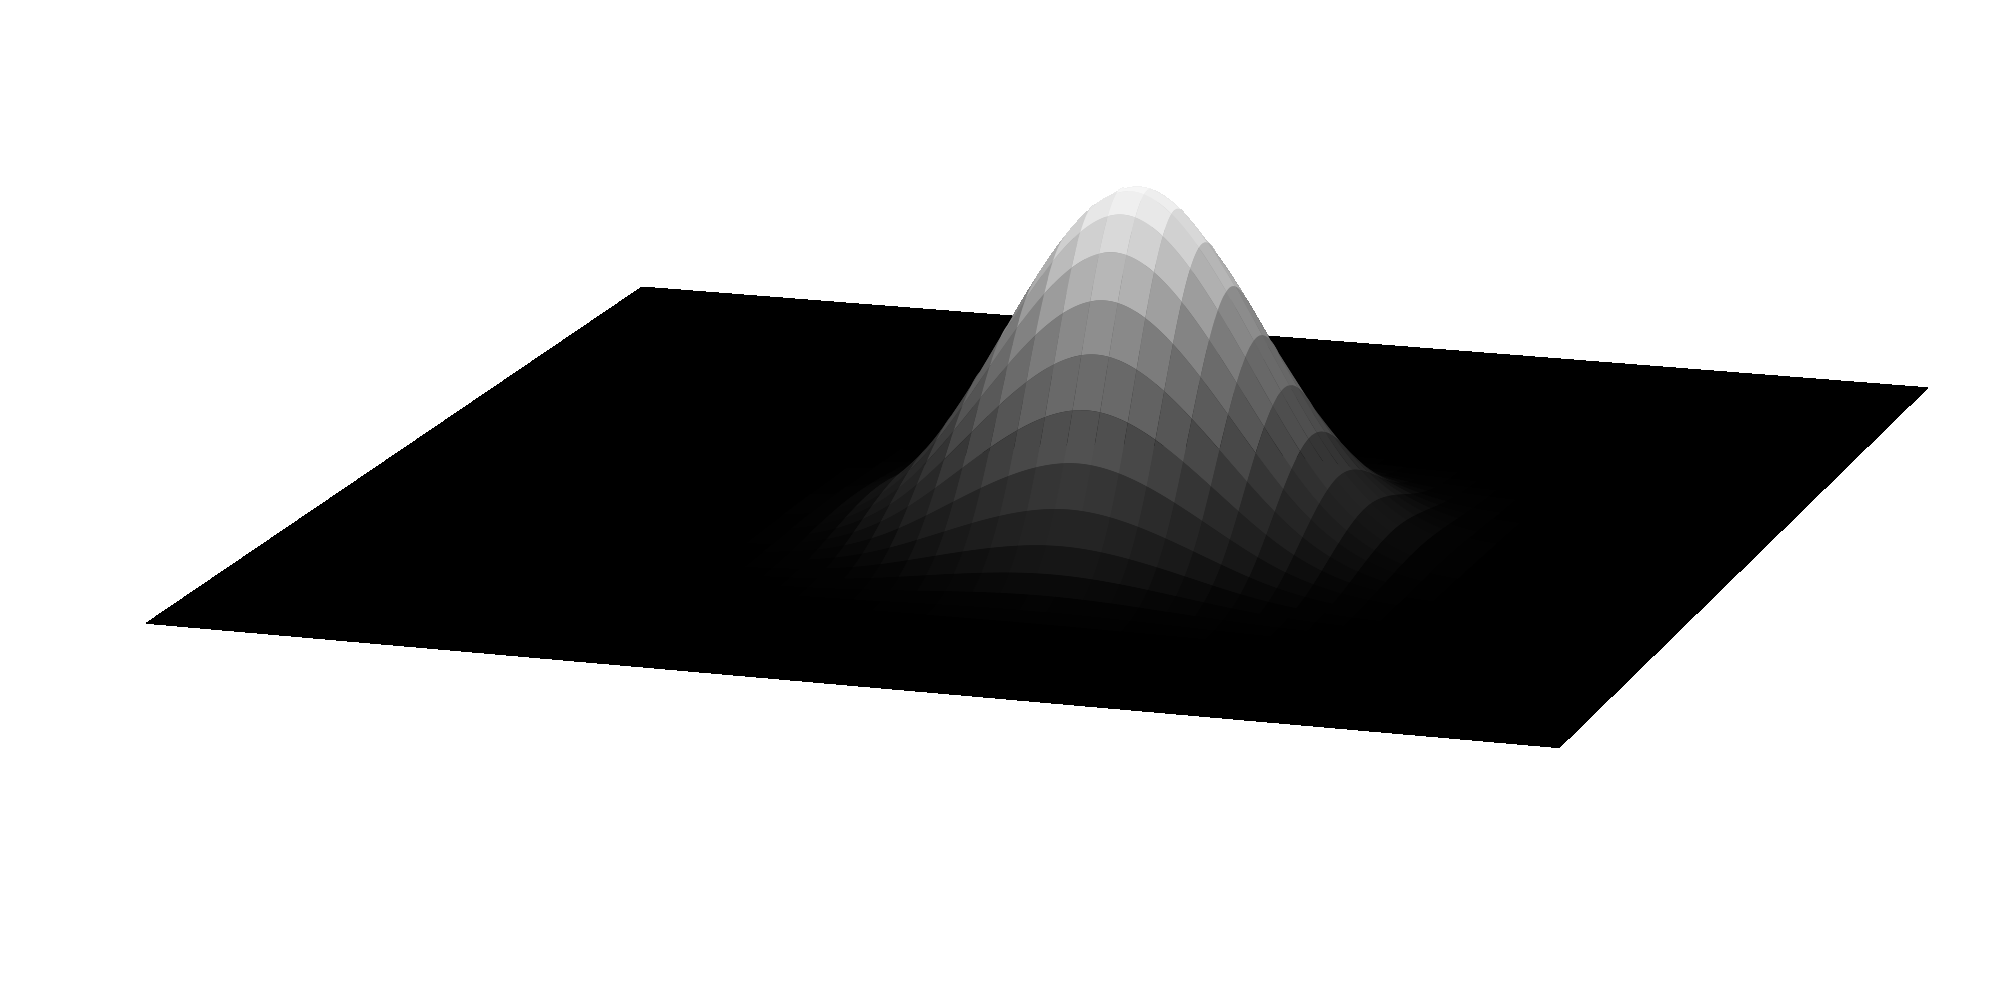
\includegraphics[width=1.0\textwidth]{images/two_dimensional_basis}
\captionsetup{labelformat=empty}
\caption{\hfill Նկար 5}
\end{figure}

\begin{figure}[h!]
\centering
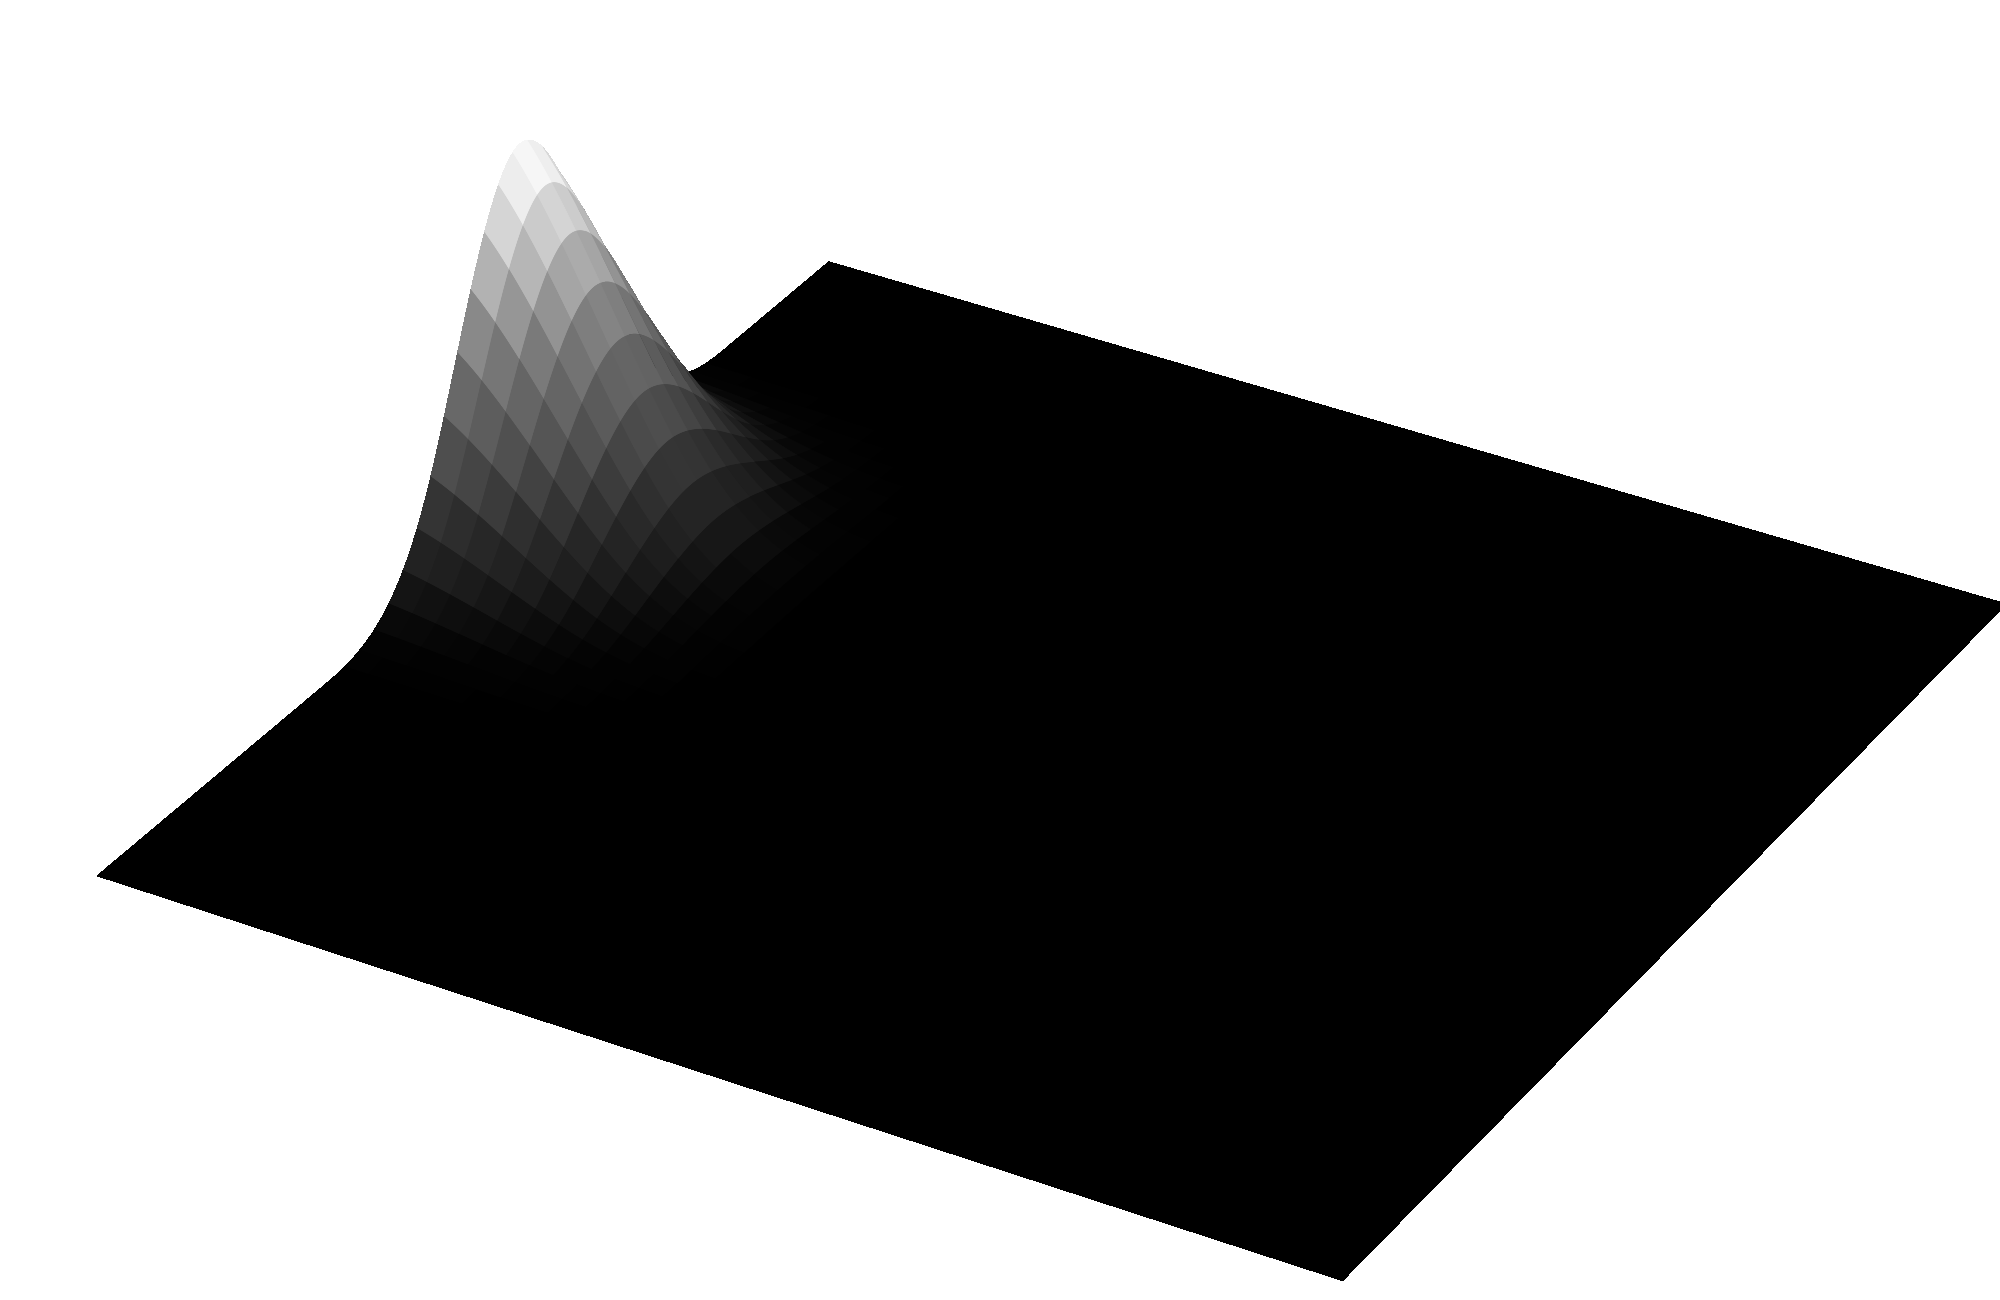
\includegraphics[width=1.0\textwidth]{images/two_dimensional_basis_1}
\captionsetup{labelformat=empty}
\caption{\hfill Նկար 5}
\end{figure}

\newpage
\subsection*{Բազմանկյուն տիրույթ}

Բազմանկյուն տիրույթ ասելով կհասկանանք կամ հենց բազմանկյունաձև տիրույթը, կամ դրա՝ բազմանկյունով մոտարկումը։ 

Դիցուք տրված են $f:\Omega\mapsto \Theta$,  $\Theta \subset \mathbb{R}$, $\Omega \subset \mathbb{R}^{2} $ բազմանկյուն տիրույթը, որը կամայական ձևով տրոհված է եռանկյուն էլեմենտների։ Յուրաքանչյուր այդպիսի $P_{1}, P_{2}, P_{3}$ գագաթներով եռանկյան համար դիտարկենք հետևյալ մոտարկող ֆունկցիան.

$$p_{1}(x, y) = \dfrac{1}{S}\sum_{i=1}^{3} p^{(1)}_{i}(x,y)f(x_{i}, y_{i})$$

$$S = \begin{vmatrix}
     1 & x_1 & y_1\\ 
     1 & x_2 & y_2\\
     1 & x_3 & y_3 
\end{vmatrix}$$

$$p^{(1)}_{i}(x,y) = x_{j}y_{k}-x_{k}y_{j}+x(y_{j}-y_{k})-y(x_{j}-x_{k})$$

\noindent որտեղ $(x_{i}, y_{i}), \; i=1, 2, 3$ տրված եռանկյուն էլեմենտի գագաթներն են (հերթականությունը ժամսլաքին հակառակ ուղղությամբ)։

\begin{figure}[h!]
\centering
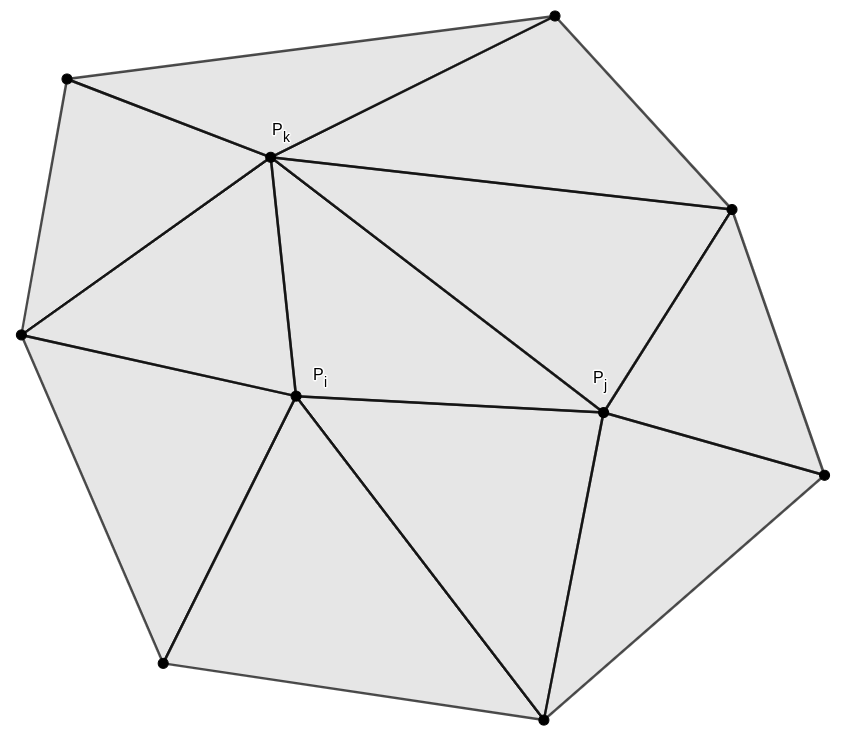
\includegraphics[width=0.4\textwidth]{images/two_var_triangular}
\captionsetup{labelformat=empty}
\caption{\hfill Նկար 6}
\end{figure}

\noindent Բնական է, որ որևէ կետի նկատմամբ լրիվ բազիսային ֆունկցիայի կառուցելու համար անհրաժեշտ է իրար գումարել այն բոլոր եռանկյուն էլեմենտների՝ այդ կետին\newline համապատասխան ֆունկցիաները, որոնց համար տվյալ կետը գագաթ է։ Հետևաբար, ընդհանուր դեպքում վերը նշված մոտարկան եղանակը հաշվողական տեսակետից հարմար չէ։

\newpage
\section*{Վարիացիոն մեթոդ}

Վարիացիոն մեթոդները հանդիպում են բազմաթիվ ֆիզիկական և այլ խնդիրնորում, և այդ խնդիրների մոտավոր լուծումը հիմնված է համապատասխան վարիացիոն մեթոդների վրա։

\subsection*{Սահմանումներ}
$f : \Omega \mapsto \Theta, \; \Omega \subset \mathbb{R}^{n}, \; \Theta \subset \mathbb{R}$ ֆունկցիայի $\epsilon$ շրջակայք ասելով կհասկանանք այն բոլոր $g$ ֆունկցիաների բազմությունը, որոնց համար տեղի ունի
$$ \left|f-g\right| < \epsilon$$
պայմանը։



\subsection*{Խնդրի դրվածքը}

Վարիացիոն մեթոդի սկզբունքն այն է, որ դիտարկվող ֆունկցիայի ինտեգրալը տրված տիրույթում ընդունում է մեծագույն (փոքրագույն) արժեք տվյալ համակարգի իրական վիճակի համար, համեմատած բոլոր հնարավոր վիճակների բազմության հետ։ \newline Ենթաինտեգրալային ֆունկցիան կախված է տրված կոորդինատներից, ֆունկցիայի արժեքից, նրա ածանցյալներից, իսկ ինտեգրումը կատարվում է տրված կոորդինատական\newline համակարգում, որը կարող է ներառել նաև ժամանակը։ Մինիմումի որոշման խնդիրը հաճախ բերվում է մի քանի դիֆերենցիալ հավասարումների, համապատասխան եզրային պայմաններով։ \newline Այն հանդիսանում է իրական փոփոխականի ֆունկցիայի էքստրեմումի որոնման խնդրի ընդհանրացում, որտեղ տվյալ ֆունկցիայի համար կոմպակտ տիրույթում անհրաժեշտ է գտնել այպիսի կետեր, որոնք հանդիսանում են մինիմում (մաքսիմում) այդ տիրույթի որևէ շրջակայքում։

Վարիացիոն մեթոդում ինտեգրալը հանդիսանում է ֆունկցիոնալ, որը կախված է ֆուկցիայից, որի որոշման տիրույթը հանդիսանում է թույլատրելի ֆունկցիաների \newline տարածությունն է։ 

Այս  մեթոդի հիմնական դժվարությունը կայանում է նրանում, որ խնդիրները, որոնք կարող են ձևակերպվել որպես վարիացիոն, հնարավոր է, որ լուծում չունենան այն պատճառով, որ ֆունկցիոնալ տարածություները  կոմպակտ չեն։

Սակայն վարիացիոն մեթոդի հիմնական առավելությունն այն է, որ դրա կիրառման համար դրվող պահանջները ավելի թույլ են, որը թույլ է տալիս միայն անընդհատ \newpage ֆունկցիաներով կառուցել մոտավոր լուծում, առանց ածանցյալների անընդհատության պայմանի։

\newpage
\subsection*{Օրինակներ}

Որպես օրինակ դիտարկենք հետևյալ կրկնակի ինտեգրալը.

$$I\left(f\right)=\iint \limits_{\Omega} F\left(x, y, f, f_{x}, f_{y}\right)dxdy$$

\noindent որտեղ $f \in C^{2}(\Omega)$,  $\Omega\subset \mathbb{R}^{2}$ և որի արժեքները որոշված են $\partial \Omega$ ում:
\noindent Այս դեպքում մինիմումի անհրաժեշտ է, որ $f(x,y)$ ֆունկցիան բավարարի Էյլեր֊Լագրանժի հավասարմանը, հավելելով համապատասխան եզրային պայմանները։

$$\dfrac{\partial}{\partial x}F_{u_{x}} + \dfrac{\partial}{\partial y}F_{u_{y}} - F_{u} = 0$$

\noindent Օրինակ, $F = \dfrac{1}{2}\left(u_{x}^2+u_{y}^2\right)$ դեպքում խնդիրը բերվում է Լապլասի հավասարմանը.

$$\dfrac{\partial^{2}f}{\partial x^{2}} + \dfrac{\partial^{2}f}{\partial y^{2}} = 0$$


Այժմ պարզ է, որ երկրորդ կարգի ածանցյալների անընդհատությունը անհրաժեշտ է Էյլեր֊Լագրանժի հավասարման գոյության համար։ Բայց վարիացիոն մեթոդը պահանջում է միայն $f$ ի անընդհատություն և առաջին կարգի մասնակի ածանցյալների կտոր առ կտոր անընդհատություն։

\subsection*{Ստացիոնար խնդիրներ} %TODO: Maybe there is another translation of word 'stationary', it would be better to use it.

Դիֆերենցիալ հավասարումը, որը կապված է վարիավիոն խնդրի հետ, կոչվում է Էյլեր֊Լագրանժի հավասարում։ Այս հանդիսանում է միայն անհրաժեշտ պայման, որին պետք է բավարարի ֆունկցիան, որը մինիմիզացնում (մաքսիմիզացնում) է ֆունկցիոնալը։ 
Դիտարկենք հետևյալ օրինակները.

\begin{enumerate}

%%%%%%%%%%%%%%%%%%%%%%%%%%%%%
\item Մեկ փոփոխականի ֆունկցիա.
$$f \in \Omega \mapsto \Theta, \; \Omega, \Theta \subset \mathbb{R}$$

\noindent Այս դեպքում ֆունկցիոնալն ընդունում է հետևյալ տեսքը.
$$I\left(f\right) = \int\limits_{x_0}^{x_{1}} F\left(x, f, f^{'}\right)dx$$

\noindent որտեղ $f(x_{0})$ և $f(x_{1})$, $x_{0}, x_{1} \in \Theta$ ը տրված են։
\noindent Մինիմիմում գոյության անհրաժեշտ պայման է հանդիսանում հետևյալ դիֆերենցիալ հավասարումը.

$$\dfrac{\partial F}{\partial f} - \dfrac{d}{dx}\dfrac{\partial F}{\partial f^{'}}=0$$
Որը համարժեք է.
$$\dfrac{d^{2}f}{dx^{2}}F_{f^{'}f^{'}}+\dfrac{df}{dx}F_{f^{'}f} + F_{f^{'}x}-F_{f}=0$$

%%%%%%%%%%%%%%%%%%%%%%%%%%%%%
\item Մի քանի անհատ ֆունկցիաներ ֆունկցիա.
$$f,g \in \Omega \mapsto \Theta, \; \Omega, \Theta \subset \mathbb{R}$$

\noindent Այս դեպքում ֆունկցիոնալն ընդունում է հետևյալ տեսքը.
$$I\left(f\right) = \int\limits_{x_0}^{x_{1}} F\left(x, f, g, f^{'}, g^{'}\right)dx$$

\noindent որտեղ $f(x_{0}), \; f(x_{1}), \; g(x_{0}), \; g(x_{1})$, $x_{0}, x_{1} \in \Theta$ ը տրված են։
\noindent Մինիմիմում գոյության անհրաժեշտ պայման է հանդիսանում հետևյալ դիֆերենցիալ հավասարումների համակարգը.

$$\dfrac{\partial F}{\partial f} - \dfrac{d}{dx}\dfrac{\partial F}{\partial f^{'}}=0$$
$$\dfrac{\partial F}{\partial g} - \dfrac{d}{dx}\dfrac{\partial F}{\partial g^{'}}=0$$

%%%%%%%%%%%%%%%%%%%%%%%%%%%%%
\item Բարձր կարգի ածանցյալներ.
$$f \in \Omega \mapsto \Theta, \; \Omega, \Theta \subset \mathbb{R}$$

\noindent Այս դեպքում ֆունկցիոնալն ընդունում է հետևյալ տեսքը.
$$I\left(f\right) = \int\limits_{x_0}^{x_{1}} F\left(x, f, f^{'}, f^{''}, \dots, f^{(n)}\right)dx$$

\noindent որտեղ $f(x_{0}), \; f(x_{1}), \; f^{'}(x_{0}), \; f^{'}(x_{1})$, $x_{0}, x_{1} \in \Theta$ ը տրված են։
\noindent Մինիմիմում գոյության անհրաժեշտ պայման է հանդիսանում հետևյալ դիֆերենցիալ հավասարումը.

$$\dfrac{\partial F}{\partial f} - \dfrac{d}{dx}\dfrac{\partial F}{\partial f^{'}} + \dfrac{d^{2}}{dx^{2}}\dfrac{\partial F}{\partial f^{''}} - \dots (-1)^{n}\dfrac{d^{n}}{dx^{n}}\dfrac{\partial F}{\partial f^{(n)}}=0$$


\item Մի քանի անկախ փոփոխականներ.
$$f \in \Omega \mapsto \Theta, \; \Omega \subset \mathbb{R}^{n}, \Theta \subset \mathbb{R}$$

\noindent Այս դեպքում ֆունկցիոնալն ընդունում է հետևյալ տեսքը.
$$I\left(f\right) = \idotsint \limits_{\Omega} F\left(x, f, f_{x_{1}}, f_{x_{2}}, \dots f_{x_{n} }\right)d\Omega$$
\noindent որտեղ $f$ ֆունկցիայի արժեքները $\partial \Omega$֊ի վրա տրված են։

\noindent Մինիմիմում գոյության անհրաժեշտ պայման է հանդիսանում հետևյալ դիֆերենցիալ հավասարումը.

$$\dfrac{\partial F}{\partial f} - \dfrac{d}{dx_{1}}\dfrac{\partial F}{\partial f_{x_{1}}} - \dots -\dfrac{d}{dx_{n}}\dfrac{\partial F}{\partial f_{x_{n}}}=0$$

\newpage
\subsubsection*{Եզրային պայմաններ}
Նախորդիվ դիտարկել էինք այնպիսի խնդիրներ, որտեղ ֆունկցիան արժեքները տրված տիրույթի եզրի տրված են։Սակայն որոշ խնդիրնորում ֆունկցիան տիրույթի եզրում տրված չէ, և տրվում են այլ տիպի եզրային պայմաններ։Նման դեպքերում որպես եզրային պայման դիտարկվում են հետևյալ պայմանները.

Մեկ փոփոխականի ֆունկցիա
$$\dfrac{\partial F}{\partial f^{'}}=0$$
Երկու անհայտ ֆունկցիա
$$\dfrac{\partial F}{\partial f^{'}}=\dfrac{\partial F}{\partial g^{'}}$$
Երկու փոփոխականի ֆունկցիա
$$F_{u_{x}}\dfrac{dy}{ds}-F_{u_{y}}\dfrac{dx}{ds}=0$$
\end{enumerate}

\noindent որոնք հայտնի են որպես \emph{բնական կամ գլխավոր}  եզրային պայմաններ։

%TODO:  add continuation from Mitchel's book from 39 to 41 pages.
\subsubsection*{Պայմանական էքստրեմում}
Այսպիսի վարիացիոն խնդիրներում անհրաշետ է մինիմիզացնել (մաքսիմիզացնել) տրված ֆունկցիոնալը, պայմանով, որ մեկ այլ ֆունկցիոնալ ընդունում է որևէ արժեք այդ ֆունկցիայի համար։ Այսինքն, եթե դիտարկենք ֆունկցիանալ, որի արժեքների բազմությունը մեկ փոփոխականի ֆունկցիաներ են, ապա կունենանք.

$$I\left(f\right)=\int \limits_{x_{0}}^{x_{1}} F\left(x, f, f^{'}\right)dx $$
$$\int \limits_{x_{0}}^{x_{1}} G\left(x, f, f^{'}\right)dx = C$$

Այս խնդրի համար Էյլեր֊Լագրանժի հավասարումը հետևյալն է.

$$\dfrac{\partial \left(F+\lambda G\right)}{\partial f} - \dfrac{d}{dx} \dfrac{\partial \left(F+\lambda G\right)}{\partial f^{'}} = 0$$


\newpage

%TODO: add description of finite elements

\section*{Մոտավոր մեթոդներ. Վերջավոր էլեմենտների մեթոդ}

Խնդիրների վարիացիոն մեթոդով ձևակերպումը, և վարիացիոն մեթոդների ավելի թույն պայմանները թույլ են տալիս այդ խնդիրները լուծել մոտավոր մեթոդներով, որոնք հաճախ անվանվում են ուղիղ մեթոդներ։ Ուղիղ մեթոդներից է Ռիտցի մինիմիզացնող հաջորդականության մեթոդը, որը քննության կառնենք։ 

\subsection*{Ռիտցի մեթոդ}

Դիտարկենք որևէ վարիացիոն մեթոդով տրված մինիմիզացիայի խնդիր.

		$$I\left(f\right) \longrightarrow min, \; f \in \Gamma$$

որտեղ $I$ ֆունկցիոնալը տրված տիրույթում որոշյալ ինտեգրալ է։

Մոտավոր լուծում կարելի է ստանալ, եթե ֆունկցիոնալի արժեքների բազմությունը սահմանափակենք որևէ վերջավոր չափանի ենթատարածությունով, որն ունի $\{\varphi_{j}\}_{j=1}^{N}$ բազիս։, 
			
			  $$\Gamma_{N} \in \Gamma $$

Ենթադրենք, որ $I$ ֆունկցիոնալի արժեքների տիրույթը ունի ճշգրիտ ստորին եզր, նշանակենք այն $\alpha_{0}$ ով։
Այդ դեպքում գոյություն ունի $\{f_{j}\}_{j=1}^{\infty}$ հաջորդականություն այնպիսին, որ

			$$ \lim_{n \to \infty}I\left(f_{n}\right) = \lim_{n \to \infty}I\left( \sum_{j=1}^{n} \gamma_{j}\varphi_{j} \right) = \alpha_{0}$$
և ֆունկցիոնալի որոշման տիրույթի ցանկացած այլ $g$ ֆունկցիայի համար
			$$I\left(g\right) \geq \alpha_{0}$$

լուծումը փնտրենք հետևյալ կերպ.

			$$f_{0}=\sum_{j=1}^{N}\gamma_{j}\varphi_{j}, \; \gamma_{j} \in \mathbb{R}$$
\noindent Այդ դեպքում խնդիրը բերվում է սովորական մինիմումի խնդրի.

   $$\dfrac{\partial I}{\partial \gamma_{i}} = \dfrac{\partial}{\partial \gamma_{i}} I \left(\sum_{j=1}^{N}\gamma_{j}\varphi_{j}\right) = 0 $$

\newpage
\subsection*{Պուասոնի հավասարման լուծում Ռիտցի մեթոդով}

Դիտարկենք հետևյալ դիֆերենցիալ հավասարումը.

				$$
					\begin{cases}
								\Delta u =f \\
								u \Big |_{\partial D} = 0
					\end{cases}
				$$
որտեղ $D = \left[x_{0}, x_{N}\right] \times \left[y_{0}, y_{M}\right]$:

Այս դիֆերենցիալ հավասարման  համապատասխան վարիացիոն խնդիրը կլինի.
			$$I(u) = \frac{1}{2}\iint \limits_{D} \left[u_x^2 + u_y^2 \right]dxdy + \iint \limits_{D} fudxdy \longrightarrow min$$

%TODO: add reference to Courant basis functions
D տիրույթը տրոհենք ուղղանկյուն եղանկյունների, և որպես բազիսային ֆունկցիաներ վերցնենք Կուրանտի ֆունկցիաները.

					$$\varphi_{i,j}(x,y)=\varphi \left(\dfrac{x-x_{i}}{h_{1}}, \dfrac{y-y_{j}}{h_{2}}\right)$$

\noindent Որոնելի ֆունկցիան կփնտրենք բազիսային ֆունկցիաների գծային կոմբինացիայի տեսքով.

					$$u(x,y) = \sum_{i=0}^{N} \sum_{j=0}^{M} u_{ij}\varphi_{i, j}(x,y)$$

\noindent  Ուստի ինտեգրալային ֆունկցիոնալը կունենա հետևյալ տեսքը.

$$\scalemath{0.9}{\frac{1}{2} \iint \limits_{D}\left[\left(\sum_{i=0}^{N} \sum_{j=0}^{M}u_{ij}\varphi_{x, ij}(x,y)\right)^2 + \left(\sum_{i=0}^{N} \sum_{j=0}^{M}u_{ij}\varphi_{y, ij}(x,y)\right)^2 \right]dxdy + \iint \limits_{D}f(x,y)\left[ \sum_{i=0}^{N} \sum_{j=0}^{M}u_{ij}\varphi_{ij}(x,y)\right]dxdy}$$

\noindent  Համաձայն էքստրեմումի անհրաժեշտ պայմանի.

$$\dfrac{\partial I}{ \partial u_{kl}} = \dfrac{\partial}{\partial u_{kl}} I \left(\sum_{j=0}^{M} u_{ij}\varphi_{i, j}(x,y)\right) = 0 $$

\noindent Դիտարկենք առաջին կրկնակի գումարը.

				$$\left(\sum_{i=0}^{N} \sum_{j=0}^{M}u_{ij}\varphi_{x, ij}(x,y)\right)^2 = u_{kl}^2\varphi_{x, kl}^2(x,y) + 2u_{kl}\varphi_{x, kl}(x,y)[\dots] + [\dots]^2$$
\noindent որտեղ բազմակետերով արտահայտությունը իր մեջ չի պարունակում $u_{kl}$ ը։

\noindent Հանգունորեն, երկրորդ կրկնակի գումարի համար՝

				$$\left(\sum_{i=0}^{N} \sum_{j=0}^{M}u_{ij}\varphi_{y, ij}(x,y)\right)^2 = u_{kl}^2\varphi_{y, kl}^2(x,y) + 2u_{kl}\varphi_{y, kl}(x,y)[\dots] + [\dots]^2$$

\noindent Այսպիսով ավելի պարզեցված տեսքով համակարգը ունի հետևյալ տեսքը.

$$\scalemath{0.85}{\frac{\partial}{\partial u_{kl}}I \left(u\right)= \iint \limits_{D} \left[2u_{kl}\varphi_{x, kl}^2(x,y) + 2\varphi_{x, kl}(x,y)[\dots] + 2u_{kl}\varphi_{y, kl}^2(x,y) + 2\varphi_{y, kl}(x,y)[\dots] + 2f(x,y)\varphi_{kl}(x,y)\right]dxdy}$$

\noindent Դիտարկենք $\varphi_{x, kl}(x,y) $ և $\varphi_{y, kl}(x,y) $ ֆունկցիաները։


$$ \varphi_{x, kl}(x,y)  = \begin{cases}
\phantom{-}0, &(x,y) \in S_{1} \\
\phantom{-}\dfrac{1}{h_{1}}, &(x,y) \in S_{2} \\
\phantom{-}\dfrac{1}{h_{1}}, &(x,y) \in S_{3} \\
\phantom{-}0, &(x,y) \in S_{4} \\
-\dfrac{1}{h_{1}}, &(x,y) \in S_{5} \\
-\dfrac{1}{h_{1}}, &(x,y) \in S_{6}\\
0, otherwise
\end{cases}, \;\; \varphi_{y, kl}(x,y)  = \begin{cases}
-\dfrac{1}{h_{2}}, &(x,y) \in S_{1} \\
-\dfrac{1}{h_{2}}, &(x,y) \in S_{2} \\
\phantom{-}0, &(x,y) \in S_{3} \\
\phantom{-}\dfrac{1}{h_{2}}, &(x,y) \in S_{4} \\
\phantom{-}\dfrac{1}{h_{2}}, &(x,y) \in S_{5} \\
0, &(x,y) \in S_{6}\\
0, otherwise
\end{cases} \;
$$

\noindent Քանի որ $\varphi_{x, kl}^2(x,y) $ և $\varphi_{y, kl}^2(x,y) $ ֆունկցիաները ոչ զրոյական են $\left[x_{k-1, l}, x_{k+1, l} \right] \times \left[y_{k, l-1}, y_{k, l+1}\right]$ ում, ապա

$$  \iint \limits_{D} 2u_{kl}\varphi_{x, kl}^2(x,y)dxdy = 4u_{kl}\dfrac{h_{2}}{h_{1}}$$
$$  \iint \limits_{D} 2u_{kl}\varphi_{y, kl}^2(x,y)dxdy = 4u_{kl}\dfrac{h_{1}}{h_{2}}$$

\noindent Քանի որ յուրաքանչյուր $\varphi_{kl}$ բազիսային ֆունկցիա հատվում Է $\varphi_{k-1, l}$, $\varphi_{k+1, l}$, $\varphi_{k, l-1}$, $\varphi_{k, l+1}$ ֆունկցիաների հետ, ապա

$$\displaylines{\iint \limits_{D} 2\varphi_{x, kl}(x,y)[\dots]dxdy = \cr
\scalemath{0.85}{2\iint \limits_{D} \varphi_{x, kl}(x,y)[u_{k-1,l}\varphi_{x, k-1, l}(x,y)+u_{k+1,l}\varphi_{x, k+1, l}(x,y)+u_{k,l-1}\varphi_{x, k, l-1}(x,y)+u_{k,l+1}\varphi_{x, k, l+1}(x,y)]dxdy =} \cr
= -2u_{k-1, l}\dfrac{h_{2} }{h_{1}} -2u_{k+1, l}\dfrac{ h_{2}}{h_{1}}}$$


 \noindent Հանգունորեն՝

			$$\scalemath{0.85}{2 \iint \limits_{D}\varphi_{y, kl}(x,y)[\dots]dxdy =  -2u_{k, l-1}\dfrac{h_{1}} {h_{2}} - 2u_{k, l+1}\dfrac{h_{1}}{ h_{2}}}$$

\noindent Եվ վերջապես

	$$ 2\iint \limits_{D} f(x,y)\varphi_{kl}(x,y)dxdy \approx 2 f_{kl} h_{1} h_{2}$$

\noindent Դիրիխլեի եզրային պայմանների համար կունենանք։
$$u_{0, l} = u_{N, l} = u_{k, 0} = u_{k, M} = 0$$

\noindent Այսպիսով, ստացանք հետևյալ հավասարումների համակարգը.

$$
\begin{cases}

			2\left[\dfrac{1}{h^{2}_{1}} + \dfrac{1}{h^{2}_{2}}\right] u_{kl}  -\dfrac{1}{h^{2}_{1}}u_{k-1, l} - \dfrac{1}{h^{2}_{1}}u_{k+1, l} -\dfrac{1}{h^{2}_{2}}u_{k, l-1} - \dfrac{1}{h^{2}_{2}}u_{k, l+1} + f_{kl} = 0\\
			u_{0, l} = u_{N, l} = u_{k, 0} = u_{k, M} = 0
\end{cases}
$$

\newpage
\subsubsection*{Ծրագրային իրականացում}

Պուասոնի հավասարման մոտավուր լուծումը իրականացնելու համար օգտվենք Python ծրագրավորմալ լեզվից, օգտագործելով Numpy գրադարանը, որը հարմար է բազմաչափ զանգվածների հետ մաթեմատիկական գործողություններ իրականացնալու համար։

Ծրագրի սկզբում տրվում է ուղղանկյուն տիրույթի սահմանները և դրա տրոհման $h_{1}$ և $h_{2}$ քայլերը, $f$ ֆունկցիան։ Հաջորդիվ կազմվում է հավասարումների համակարգը, կանչվում այն լուծող ֆունկցիան։ Այսնուհետև բազիսային ֆունկցիաների միջոցով կառուցվում է մոտարկող ֆունկցիան։

Օրինակ


				$$
					\begin{cases}
								\Delta u =2 \\
								u \Big |_{\partial D} = 0
					\end{cases}
				$$

				$$ D = \left[-\dfrac{\pi}{2}, \phantom{-}\dfrac{\pi}{2}\right] \times \left[-\dfrac{\pi}{2}, \phantom{-}\dfrac{\pi}{2}\right], \; h_{1}=h_{2}=\dfrac{\pi}{200}$$

\noindent Խնդրի համար ստացված լուծումը.

\begin{figure}[h!]
\centering
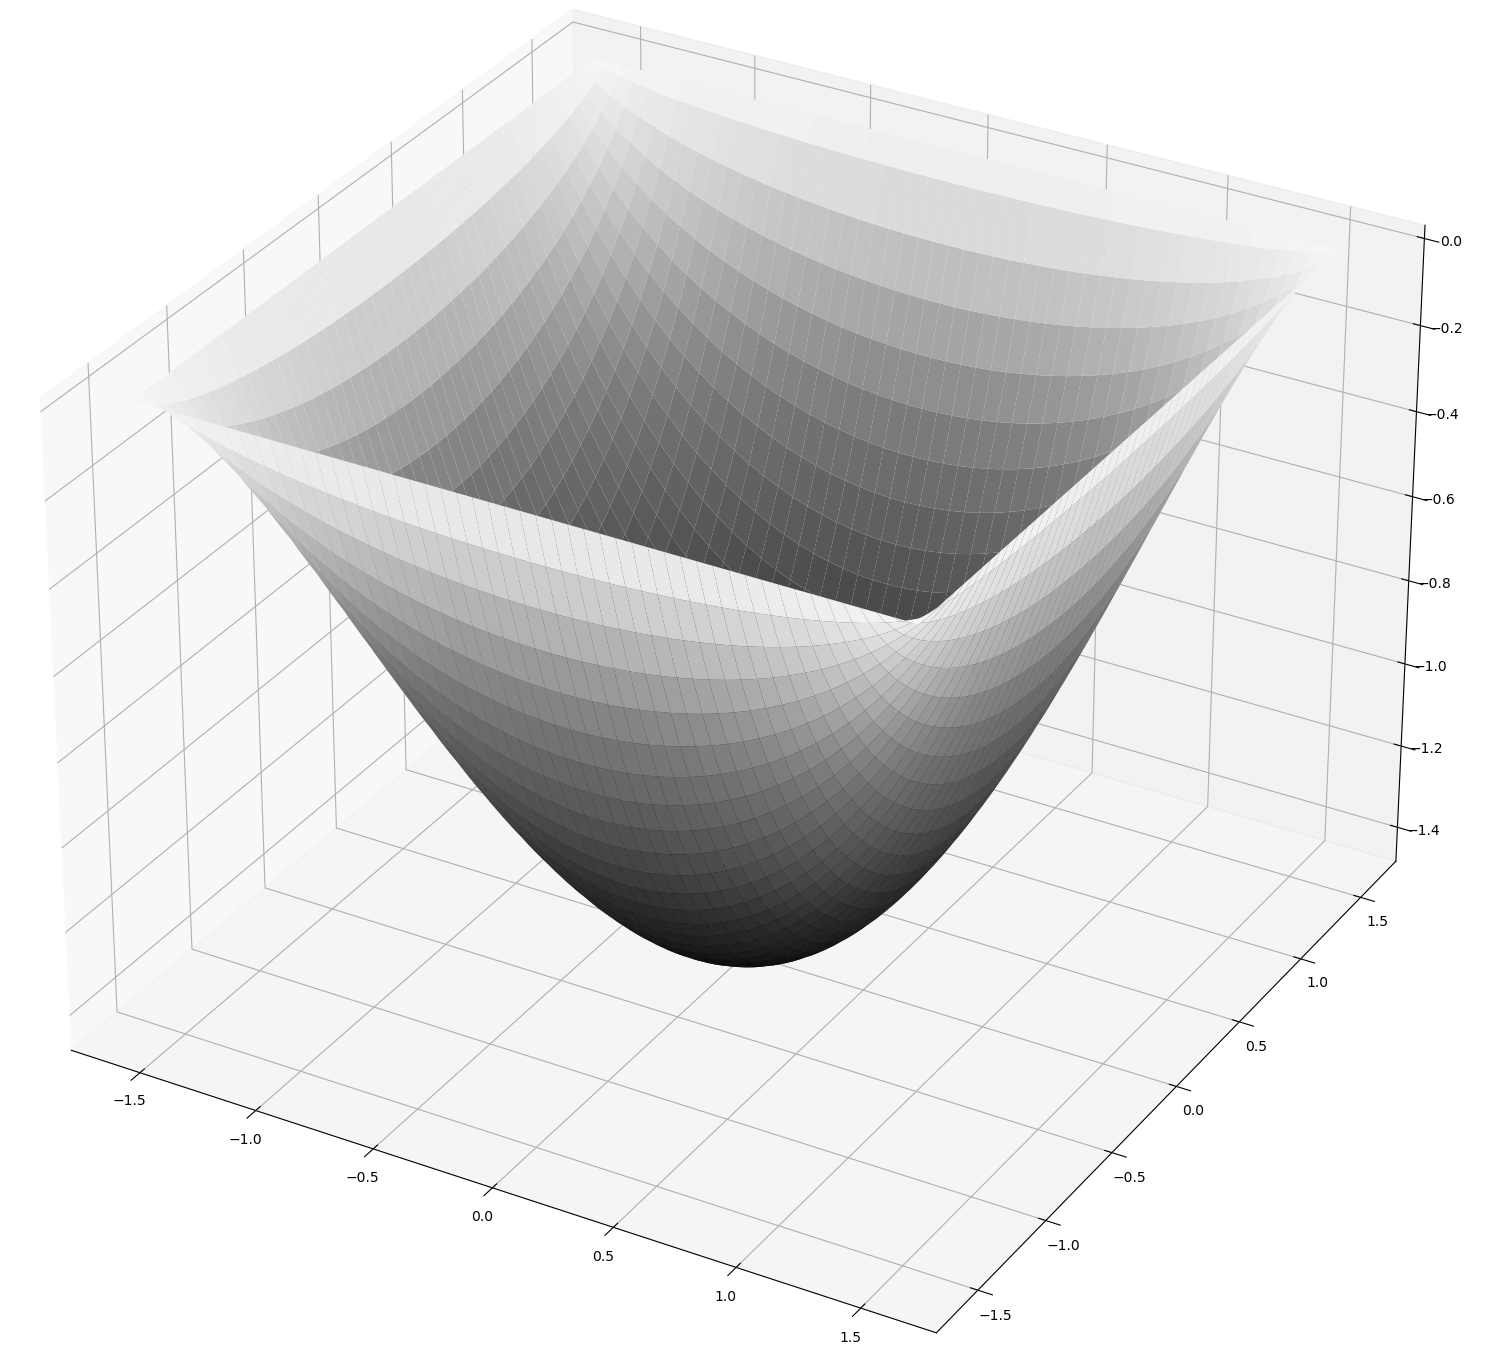
\includegraphics[width=0.9\textwidth]{images/poisson_solution}
\captionsetup{labelformat=empty}
\caption{\hfill Նկար 7}
\end{figure}

\subsection*{Բիհարմոնիկ հավասարում}

Դիտարկենք հետևյալ դիֆերենցիալ հավասարումը.

$$\begin{dcases}
								\Delta^{2} u &=f \\
								u \Big |_{\partial D} &= 0\\
								\dfrac{\partial u}{\partial n} \Big |_{\partial D} &= 0
\end{dcases}$$
որտեղ $D = \left[x_{0}, x_{N}\right] \times \left[y_{0}, y_{M}\right]$:

Այս դիֆերենցիալ հավասարման  համապատասխան վարիացիոն խնդիրը կլինի.
			$$I(u) = \frac{1}{2}\iint \limits_{D} \left[u_{xx}^{2} + 2u_{xy}^{2} + u_{yy}^{2} \right]dxdy + \iint \limits_{D} fudxdy \longrightarrow min$$

$D$ տիրույթը տրոհենք ուղղանկյուների $h_{1}$ և $h_{2}$ քայլերով համապատասխանաբար ըստ $x$ և $y$ կոորդինատների։
\noindent Որոնելի ֆունկցիան կփնտրենք բազիսային ֆունկցիաների գծային կոմբինացիայի տեսքով.

					$$u(x,y) = \sum_{i=0}^{N} \sum_{j=0}^{M} u_{ij}\varphi^{ij}(x,y)$$
\noindent Հետևաբար ինտեգրալ ֆունկցիոնալը կունենք հետևյալ տեսքը.

$$\scalemath{0.7}{\frac{1}{2} \iint \limits_{D}\left[\left(\sum_{i=0}^{N} \sum_{j=0}^{M}u_{ij}\varphi^{ij}_{xx}(x,y)\right)^2 +  2\left(\sum_{i=0}^{N} \sum_{j=0}^{M}u_{ij}\varphi^{ij}_{xy}(x,y)\right)^2 + \left(\sum_{i=0}^{N} \sum_{j=0}^{M}u_{ij}\varphi^{ij}_{yy}(x,y)\right)^2\right]dxdy + \iint \limits_{D}f(x,y)\left[ \sum_{i=0}^{N} \sum_{j=0}^{M}u_{ij}\varphi^{ij}(x,y)\right]dxdy}$$


\noindent  Համաձայն էքստրեմումի անհրաժեշտ պայմանի.

$$\dfrac{\partial I}{ \partial u_{kl}} = \dfrac{\partial}{\partial u_{kl}} I \left(\sum_{j=0}^{M} u_{ij}\varphi^{ij}(x,y)\right) = 0 $$


\noindent Դիտարկենք առաջին կրկնակի գումարը.
$$\left(\sum_{i=0}^{N} \sum_{j=0}^{M}u_{ij}\varphi_{xx}^{ij}(x,y)\right)^2 = \left[u_{kl}\varphi_{xx}^{kl}(x,y)\right]^{2} + 2u_{kl}\varphi_{xx}^{kl}(x,y)[\dots] + [\dots]^2$$
\noindent որտեղ բազմակետերով արտահայտությունը իր մեջ չի պարունակում $u_{kl}$ ը։
Հանգունորեն երկրորդ կրկնակի գումարի համար.
$$\left(\sum_{i=0}^{N} \sum_{j=0}^{M}u_{ij}\varphi_{xy}^{ij}(x,y)\right)^2 = \left[u_{kl}\varphi_{xy}^{kl}(x,y)\right]^{2} + 2u_{kl}\varphi_{xy}^{kl}(x,y)[\dots] + [\dots]^2$$
Հանգունորեն երրորդ կրկնակի գումարի համար.
$$\left(\sum_{i=0}^{N} \sum_{j=0}^{M}u_{ij}\varphi_{yy}^{ij}(x,y)\right)^2 = \left[u_{kl}\varphi_{yy}^{kl}(x,y)\right]^{2} + 2u_{kl}\varphi_{yy}^{kl}(x,y)[\dots] + [\dots]^2$$



\noindent Այսպիսով ավելի պարզեցված տեսքով համակարգը ունի հետևյալ տեսքը.

$$\scalemath{0.65}{\frac{\partial}{\partial u_{kl}}I \left(u\right)= \iint \limits_{D} \left[2u_{kl}\left\{ \varphi_{xx}^{kl}(x,y)\right\}^{2} + 2\varphi_{xx}^{kl}(x,y)[\dots] + 4u_{kl}\left\{ \varphi_{xy}^{kl}(x,y)\right\}^{2} + 4\varphi_{xy}^{kl}(x,y)[\dots] + 2\left\{ \varphi_{yy}^{kl}(x,y)\right\}^{2} + 2u_{kl}\varphi_{yy}^{kl}(x,y)[\dots] + 2f(x,y)\varphi_{kl}(x,y)\right]dxdy}$$

Քանի որ տրված են Դիրիխլեի և Նեյմանի եզրային պայմանները, կդիտարկենք միայն $2 \leq k \leq M-2, 2 \leq l \leq N-2$ դեպքերը։ 

\noindent Ինտեգրալը հաշվենք անդամ առ անդամ։

$$\iint \limits_{D} 2u_{kl}\left\{ \varphi_{xx}^{kl}(x,y)\right\}^{2}dxdy=2u_{kl}\int \limits_{x_{k-2}}^{x_{k+2}}\int \limits_{y_{l-2}}^{y_{l+2}} \left\{ B_{k}^{''}(x)B_{l}(y)\right\}^{2}dxdy=2u_{kl}\cdot \dfrac{6}{h_{1}^{3}} \cdot \dfrac{151}{140}h_{2}$$
$$\iint \limits_{D} 4u_{kl}\left\{ \varphi_{xy}^{kl}(x,y)\right\}^{2}dxdy=4u_{kl}\int \limits_{x_{k-2}}^{x_{k+2}}\int \limits_{y_{l-2}}^{y_{l+2}} \left\{ B_{k}^{'}(x)B_{l}^{'}(y)\right\}^{2}dxdy=4u_{kl}\cdot \dfrac{3}{2h_{1}} \cdot \dfrac{3}{2h_{2}}$$
$$\iint \limits_{D} 2u_{kl}\left\{ \varphi_{yy}^{kl}(x,y)\right\}^{2}dxdy=2u_{kl}\int \limits_{x_{k-2}}^{x_{k+2}}\int \limits_{y_{l-2}}^{y_{l+2}} \left\{ B_{k}(x)B_{l}^{''}(y)\right\}^{2}dxdy=2u_{kl}\cdot \dfrac{151}{140}h_{2} \cdot \dfrac{6}{h_{1}^{3}}$$

Քանի որ $\varphi^{ij}$ բազիսային ֆունկցիաները ունեն լոկալ կրողներ $4 \times 4 = 16$ ուղղանկյուն էլեմենտներում, ապա տրված $\varphi^{kl}$ ֆունկցիան հատվում է 49 այլ բազիսային ֆունկցիաների հետ։

\begin{figure}[h!]
\centering
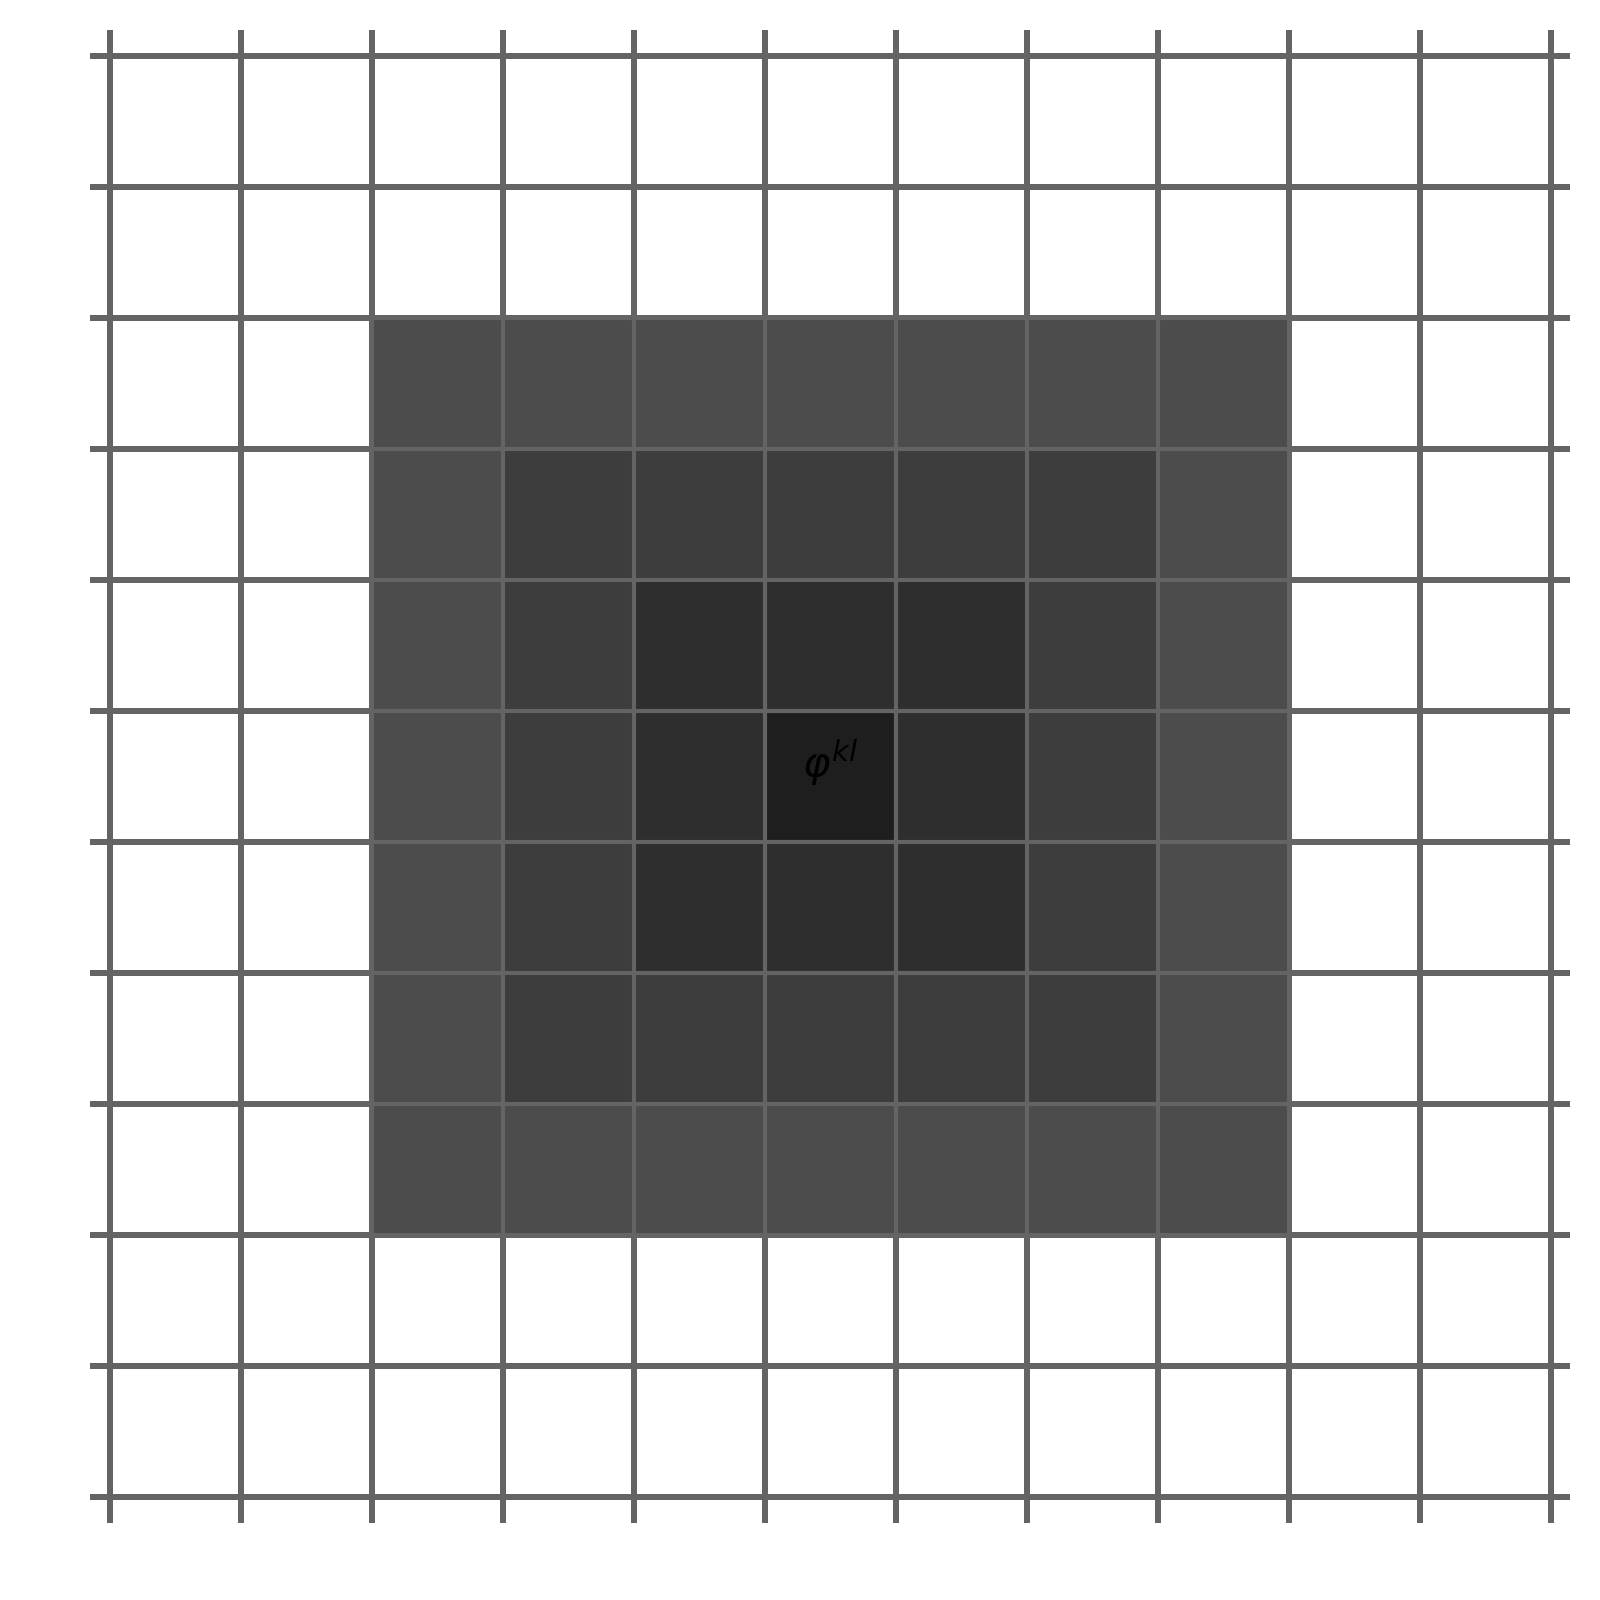
\includegraphics[width=0.3\textwidth]{images/two_dimensional_basis_intersection}
\captionsetup{labelformat=empty}
\caption{\hfill Նկար 7}
\end{figure}

Ստորև ներկայացվում են 
		$$\iint \limits_{D} 2\varphi_{xx}^{kl}(x,y)[\dots]dxdy, \iint \limits_{D} 4\varphi_{xy}^{kl}(x,y)[\dots]dxdy, \iint \limits_{D} 2\varphi_{yy}^{kl}(x,y)[\dots]dxdy$$

\noindent ինտեգրալների արժեքները աղյուսակի տեսքով.

$$\iint \limits_{D} 2\varphi_{xx}^{kl}(x,y)[\dots]dxdy= 2\sum_{\substack{i=k-3\\ i \neq k}}^{k+3}\sum_{\substack{j=l-3\\ j \neq l}}^{l+3} u_{ij}\int \limits_{x_{k-2}}^{x_{k+2}}B_{k}^{''}(x)B_{i}^{''}(x)dx \int \limits_{y_{l-2}}^{y_{l+2}}B_{l}(x)B_{j}(x)dy$$
$$\iint \limits_{D} 4\varphi_{xy}^{kl}(x,y)[\dots]dxdy= 4\sum_{\substack{i=k-3\\ i \neq k}}^{k+3}\sum_{\substack{j=l-3\\ j \neq l}}^{l+3}u_{ij}\int \limits_{x_{k-2}}^{x_{k+2}}B_{k}^{'}(x)B_{i}^{'}(x)dx \int \limits_{y_{l-2}}^{y_{l+2}}B_{l}^{'}(x)B_{j}^{'}(x)dy$$
$$\iint \limits_{D} 2\varphi_{yy}^{kl}(x,y)[\dots]dxdy= 2\sum_{\substack{i=k-3\\ i \neq k}}^{k+3}\sum_{\substack{j=l-3\\ j \neq l}}^{l+3}u_{ij}\int \limits_{x_{k-2}}^{x_{k+2}}B_{k}(x)B_{i}(x)dx \int \limits_{y_{l-2}}^{y_{l+2}}B_{l}^{''}(x)B_{j}^{''}(x)dy$$

\begin{figure}[h!]
\centering
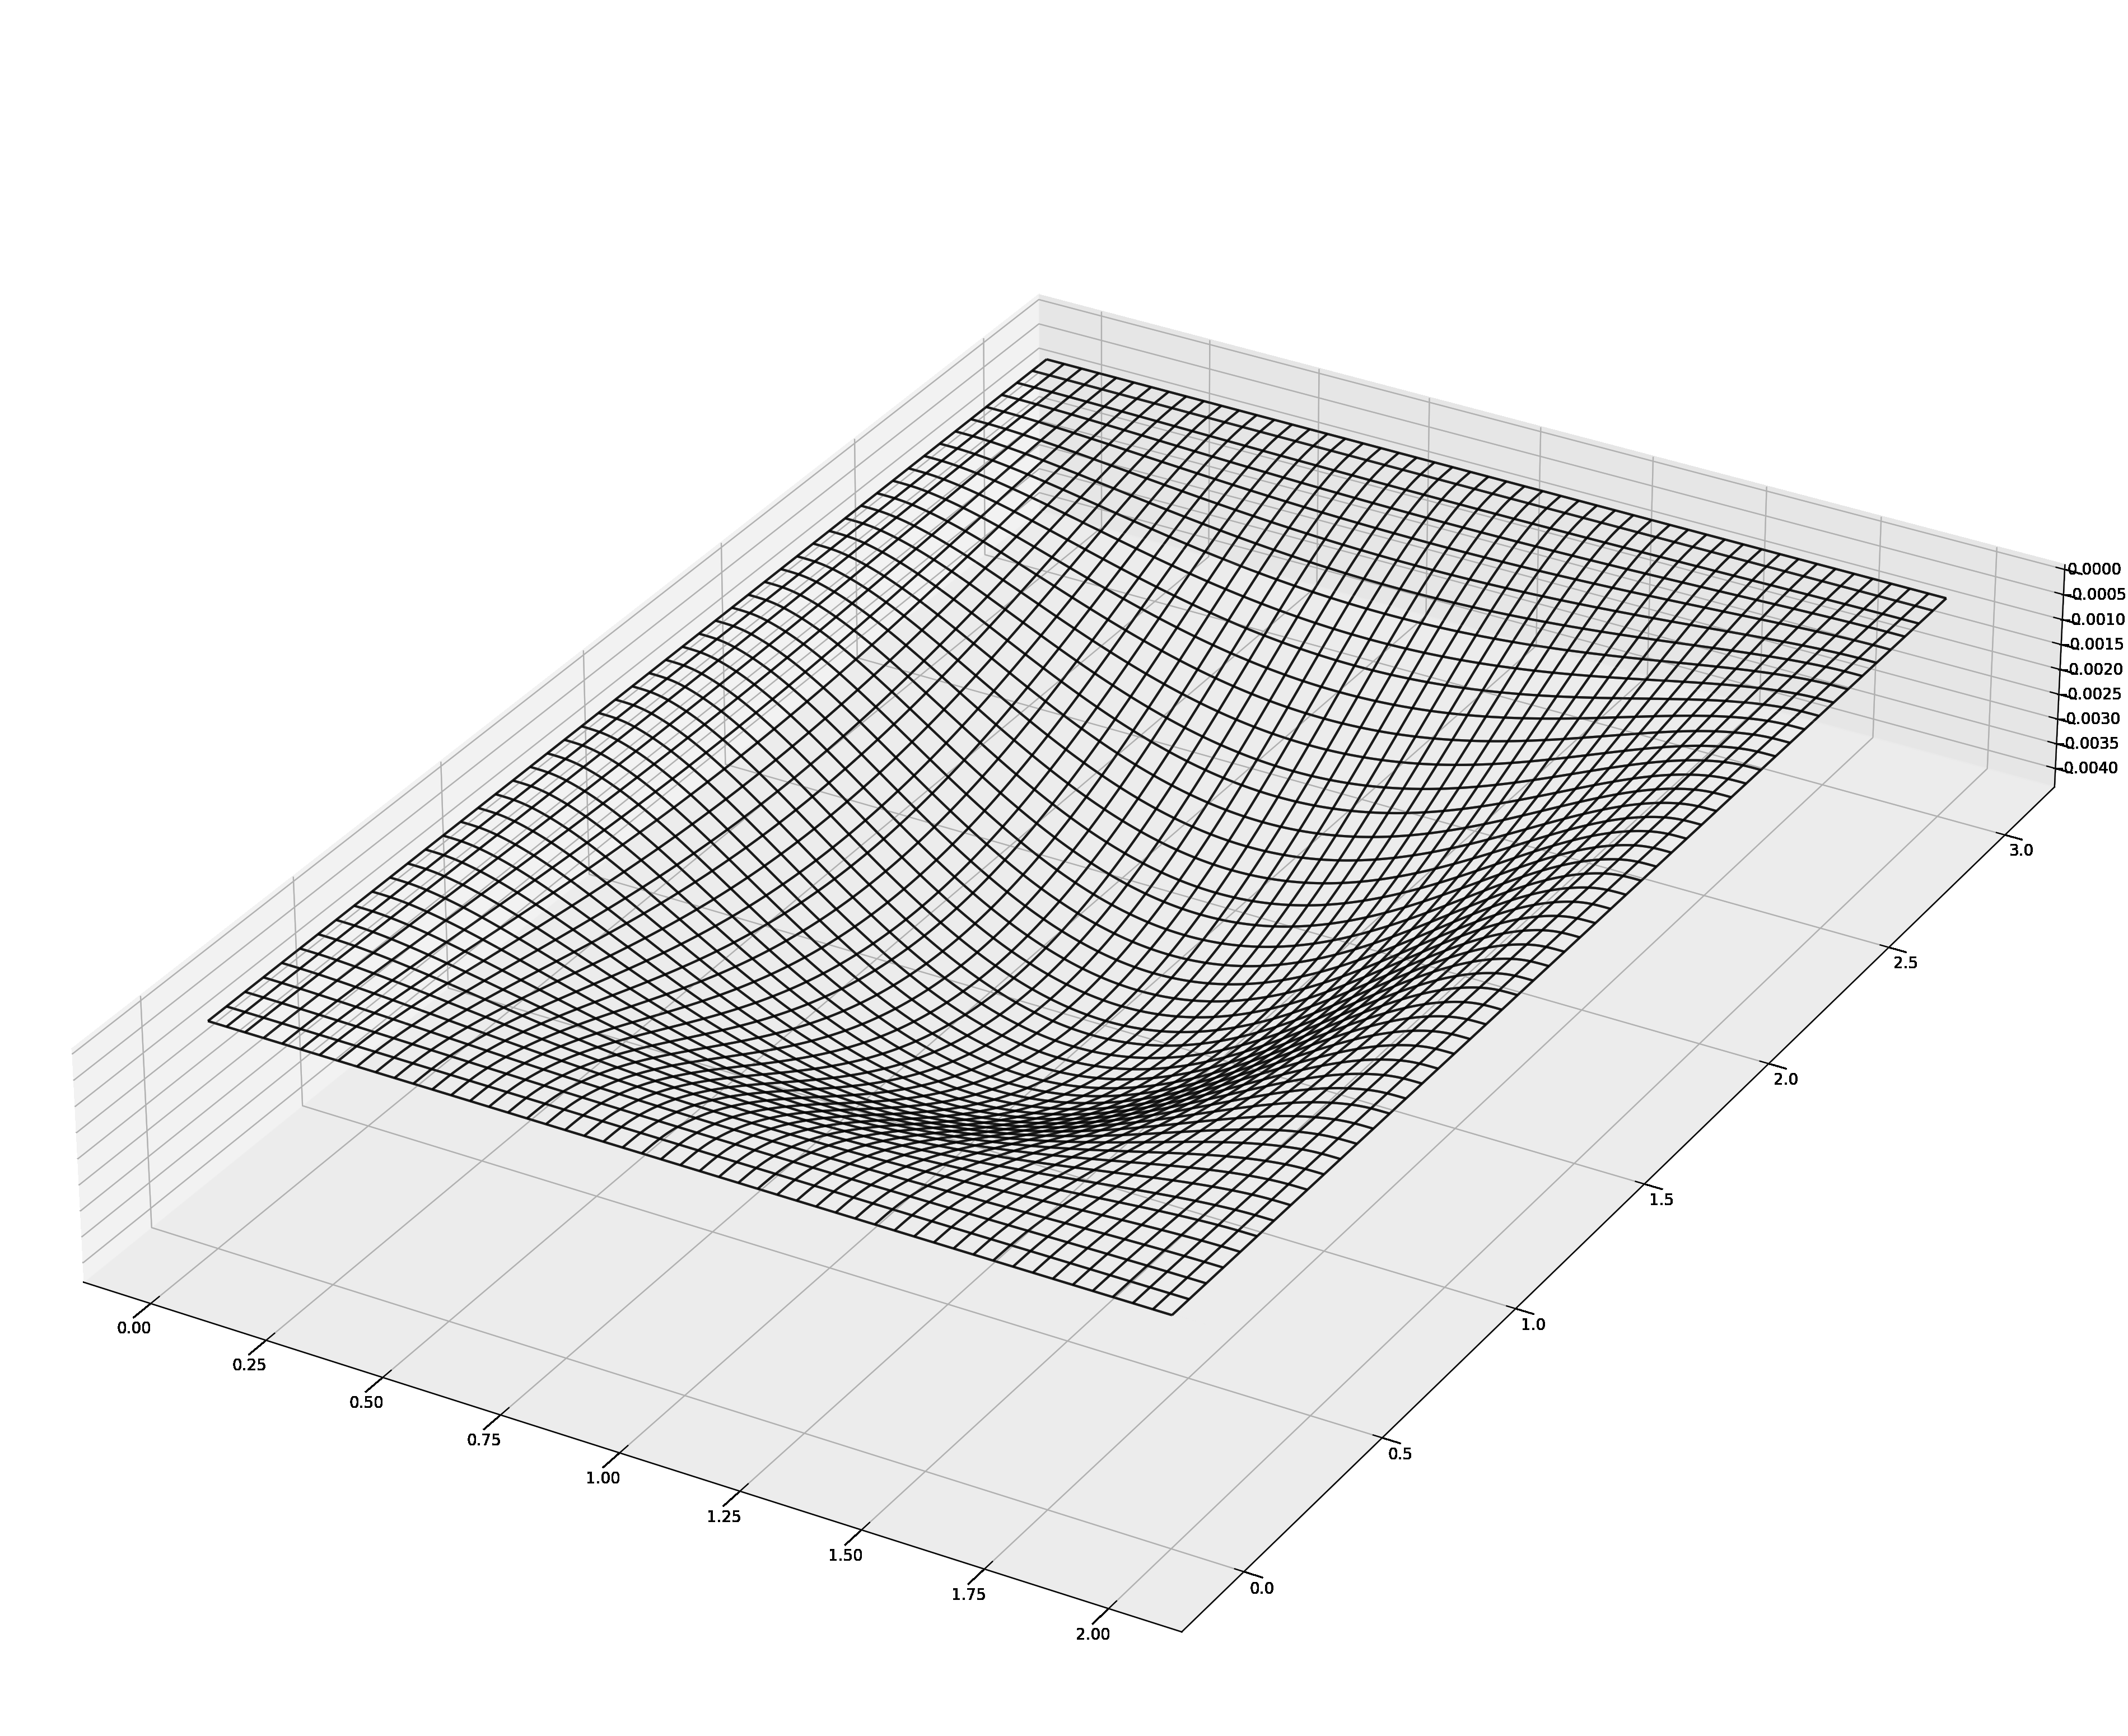
\includegraphics[width=0.9\textwidth]{images/biharmonic_equation_solution}
\captionsetup{labelformat=empty}
\caption{\hfill Նկար 7}
\end{figure}


\end{document}